\documentclass{article}

\usepackage{arxiv}

\usepackage[utf8]{inputenc} % allow utf-8 input
\usepackage[T1]{fontenc}    % use 8-bit T1 fonts
\usepackage{lmodern}        % https://github.com/rstudio/rticles/issues/343
\usepackage{hyperref}       % hyperlinks
\usepackage{url}            % simple URL typesetting
\usepackage{booktabs}       % professional-quality tables
\usepackage{amsfonts}       % blackboard math symbols
\usepackage{nicefrac}       % compact symbols for 1/2, etc.
\usepackage{microtype}      % microtypography
\usepackage{graphicx}

\title{Ownership dynamics, risk and regulation in Chinese banking: New Evidence}

\author{
    Veronica Zhang
    \thanks{The authors gratefully acknowledge Professor John Turner and Dr Clive
Walker for their insight comments.}
   \\
    Management School, Queen's University Belfast \\
   \\
  \texttt{} \\
   \And
    Lisa Sheenan
   \\
    Management School, Queen's University Belfast \\
   \\
  \texttt{} \\
   \And
    Barry Quinn
   \\
    Management School, Queen's University Belfast \\
   \\
  \texttt{} \\
  }



% Pandoc citation processing

\usepackage{longtable}
\usepackage{color}
\usepackage{xcolor}
\usepackage{multirow}
\usepackage{multicol}
\usepackage{colortbl}
\usepackage{hhline}
\usepackage{longtable}
\usepackage{array}
\usepackage{hyperref}


\begin{document}
\maketitle

\def\tightlist{}


\begin{abstract}
Enter the text of your abstract here.
\end{abstract}

\keywords{
    Chinese financial institutions
   \and
    Industrial organisation
   \and
    State ownership
   \and
    Credit risk
  }

\hypertarget{introduction}{%
\section{Introduction}\label{introduction}}

\label{sec:intro}

The relationship between capital buffers and bank risk-taking has long
attracted academic attention, (Cooper and Ross 2002; Demirgüç-Kunt and
Kane 2002; Keeley 1990). The implementation of Basel Accords also lead
to work focusing on the effects of capital regulation on bank behaviour,
in particular on the impact of capital adequacy requirements on bank
risk-taking behaviour. The 2007-2009 global financial crisis uncovered
structural weaknesses in capital regulations which were implemented
before the crisis. After the crisis, the Basel Committee on Banking
Regulation and Supervision (BCBS) developed a consolidated framework
(Basel III) for more stringent capital adequacy regulations and
liquidity assessment, in recognition of the need for banks to be subject
to more stringent capital regulations. Following the goals set by the
BCBS, member countries, including China, have established legislation
and regulatory frameworks. While regulatory consensus has been reached
focusing on capital buffers, there is continued academic debate about
what effect capital requirements could have on bank risk-taking
(Chiaramonte and Casu 2017; Demirguc-Kunt, Detragiache, and Merrouche
2013; Roulet 2018)

China's banking sector plays an essential role in the country's economic
development. It underwent fundamental reform in 1978, as an integrate
part of China's overall economic reform. Since 2001, when China got
accession to the World Trade Organization (WTO), the reform of China's
banking system has stepped up its pace and the whole banking sector has
been dramatically reshaped. The reform has transformed Chinese banks
into market-oriented enterprises, changed their ownership structure,
established modern corporate governance mechanisms, and introduced
legislation and regulatory framework. Since 2010, improvements and
refinements have continued in China's banking sector as part of an
advanced stage of the reform. China's financial authority fully accepted
the Basel III framework and began its implementation in 2013. A rich
body of literature focusing on the previous stages of the reform
assesses the relationship between capital requirements and Chinese
banks' performance and risk-taking (T.-H. Lee and Chih 2013; Pessarossi
and Weill 2015; Tan and Floros 2013). The objective of this paper is to
analyze the impact of capital requirements on Chinese bank risk-taking
following the 2007-2009 global financial crisis using the risk-based
capital definition of the Basel III framework.

In this paper, we extend existing empirical work studying the impact of
capital requirements on bank credit risk-taking by incorporating the
interaction between capital regulation and ownership structure.
Financial theories suggest that capital regulations impact banks'
risk-taking due to the effect of the regulation on shareholders'
incentives. (Allen, Carletti, and Marquez 2011; Demirgüç-Kunt and Kane
2002) (Demirgüç-Kunt and Kane, 2002, Allen et al., 2011) Empirical
studies support those theories. Nevertheless, empirical studies find
mixed results including negative association {[}RN24;RN75{]} (Berger and
Bouwman, 2013, Tan and Floros, 2013), positive association {[}RN27{]}
(Bichsel and Blum, 2004) and nonlinear relationships (Calem and Rob
1999) between capital regulation and bank risk-taking. Agency theory
suggests that corporate risk-taking is influenced by ownership structure
depending on the power of shareholder control. (Jensen and Meckling
1976, @RN4) Therefore, these theoretical keystones provide the
foundation for us to examine the effect of capital regulation on bank
risk-taking and how this interacts with ownership structure in
determining risk-taking.

This paper provides empirical evidence using forensically analysed data
on 231 China's commercial banks over the period 2010-2019. To perform
our analysis, we also hand collect the ownership structure information
of these 231 Chinese commercial banks and classify them into 5
categories of ownership identities: State-owned (Big Six and other than
Big Six), Local government-holding, Joint-stock, Foreign joint-stock,
and Foreign-owned banks. (Table 1) We regress both regulatory capital
requirements from the Basel III framework and ownership identities on
bank credit risk-taking proxies, respectively. We employ banks'
Non-performing Loans (NPL) ratios and Loan Loss Reserves (LLR) ratios to
reflect the level of banks' credit risk-taking. We also examine the
actual impact of Basel III capital regulation on credit risk-taking
incorporating the interaction between capital regulation and ownership
structure.

Our key findings are as follows. First, credit risk is generally lower
in banks that have higher regulatory capital. This finding is consistent
with the theory suggesting regulatory capital acts as a buffer to resist
economic shocks and lower banks' risk-taking incentives (Demirguc-Kunt,
Detragiache, and Merrouche 2013, @RN64). This finding also supports the
empirical studies of Chinese banks conducted by Tan and Floros (2013)
and Lee, Ning, and Lee (2015).

Second, state-owned banks in gene1ral have higher credit risk compared
to foreign-owned banks and other ownership identities. This finding is
consistent with the results of Zhu and Yang (2016) which examines
risk-taking of state-owned banks and foreign banks. This finding also,
to some extent, backs up the empirical results of Laeven and Levine
(2009) which finds banks with large owners who have significant cash
flow rights take higher credit risk. During the financial reform, the
state-shareholder in Chinese banks has transformed from a state-bureau
(e.g., the Finance Ministry) to a state-corporation (e.g., Central
Huijin Investment Co.) with modern corporate governance mechanisms. The
state-shareholder has become a shareholder with \emph{highly
concentrated control rights and significant cash flow rights}. Due to
this fact, our finding can be considered consistent with the agency
theory that concentrated ownership and powerful shareholders suggest
higher corporate risk-taking(Saunders, Strock, and Travlos 1990; Stulz
2005). This finding also supports the social view of the theory of state
ownership of banks that state-owned banks would undertake credit
projects which might not be financially profitable(Stiglitz 1993).

Third, the actual impact of Basel III capital regulation on credit
risk-taking can be influenced, to some extent, by ownership structure.
For example, the results suggest that in government-holding banks, the
negative effect of capital regulation on credit risk-taking can be
enhanced by its ownership identity when there is no shareholder with
significant power to increase risk-taking incentives.

This paper contributes to the literature in several ways. First, this
study assesses the impact of risk-based capital regulation on Chinese
bank credit risk-taking following the global financial crisis, using the
definition of capital from Basel III framework. It has been 10 years
since the BCBS first released Basel III framework in 2010. The Chair of
the BCBS stated that evaluating the regulation effects is part of the
BCBS post-crisis reform in the current macroeconomic environment. In
addition, China's banking industry achieved extensive transformation
before 2010 and the Chinese case provides uniqueness in terms of
ownership structure.

Second, our study bridges the research gap by incorporating the
interaction between ownership structure and capital regulation while
examining the impact of Basel III capital requirements on bank credit
risk-taking. Only a small number of existing studies evaluate the joint
effects of ownership structure and bank regulations on bank risk-taking,
such as Laeven and Levine (2009) 2009. Pessarossi and Weill (2015) test
the impact of the interaction between capital regulation and ownership
structure on cost efficiency of Chinese banks. To the best of our
knowledge, this is the first study to assess how Basel III regulation
and ownership structure jointly shape Chinese bank credit risk-taking
following the global financial crisis.

Third, we analyse a bespoke dataset of 231 Chinese commercial banks over
a relatively long period (2010-2019) to study China's banking sector.
These 231 banks account for over 80\% of China's banking sector in terms
of total assets. Apart from employing the data provided by the SNL
database, we hand collected any missing values from the original annual
reports of individual banks, which makes our data set extremely
comprehensive.

The remainder of this paper is organised as follows. Section II reviews
related literature, develops the testable predictions, as well as a
brief introduction of the evolution of ownership structure of commercial
banks in China. Section III presents the data set and the empirical
model including the variables considered in our analysis. The empirical
results are presented in section IV. And section V concludes.

\hypertarget{literature}{%
\section{Literature}\label{literature}}

As a member of the G20 and the Basel Committee on Banking Supervision,
China has been fully supporting and participating in the global
regulatory reform following the Great Financial Crisis of 2007-2009. In
June 2012, The China Banking Regulatory Commission (CBRC) issued the
regulation \emph{Commercial Bank Capital Management Measure (Trial)},
which means that the Basel III framework was adopted and incorporated
into the banking regulatory framework in China. The relationship between
macro and micro prudential regulations has a hierarchical structure.
Borio (2003) argue that the objectives of macro-prudential regulation
subsume the rationales of the micro-prudential approach. The Basel III
Framework is a macro-prudential framework based on Basel II framework (a
micro-prudential framework). Through examining the relation between
credit risk/solvency risk and Basel III, the impact of this
macro-prudential oriented framework can be assessed from the
institutional angle.

\hypertarget{bank-capital-and-risk}{%
\subsection{Bank capital and risk}\label{bank-capital-and-risk}}

Empirical literature and financial theories provide mixed views
regarding the impact of bank capital on risk-taking and bank stability.
The Basel framework, centered with capital regulation, is designed to
reduce bank risk and enhance bank resilience. Anginer and Demirguc-Kunt
(2014) support this view that bank capital acts as a buffer in absorbing
economic shocks and strengthens systemic stability. Demirguc-Kunt,
Detragiache, and Merrouche (2013) find that a strong capital position
helps banks resist earning shocks and have higher probability to survive
the crisis. They also find evidence to advocate higher quality capital,
i.e., Tier 1 capital, in the regulatory capital requirements. A lot of
theories underline that risk-based capital, more effective than interest
rate ceilings, boosts banks' ``franchise value'', improve borrowers
screening, and lower banks' excessive risk-taking incentives {[}Allen,
Carletti, and Marquez (2011);RN64;RN67{]}. Other theories emphasize a
moral hazard perspective, arguing effective regulatory capitalization
may offset the excessive risk-taking incentives created by deposit
insurance (Keeley 1990; Demirgüç-Kunt and Kane 2002). In terms of
Chinese commercial banks, (Tan and Floros 2013) find a significant
negative relationship between bank capital and risk. ({\textbf{???}})
report that bank capital is negatively related to NPL and support
theories with the moral hazard view.

Contrariwise, other research posits that greater capital regulations may
induce higher bank risk. Cooper and Ross (2002) extend the research of
Diamond and Dybvig (1983), stating that the existence of deposit
insurance weaken the depositors' incentive to monitor banks and causes
them to engage in excessive risk-taking activities. Blum (1999) suggests
that banks may have higher incentives to raise risk due to the binding
capital adequacy requirements. Calem and Rob (1999) find a U-shaped
relationship between bank capital position and risk. The risk-taking
first decreases with the increase of bank capital; then it increases as
bank capital increases on its high level. They also argue that the
increase in capital adequacy requirements induces banks to take
additional portfolio risk even if they are well-capitalized. For Chinese
banking data, T.-H. Lee and Chih (2013) find that the negative
relationship between capital and risk only exists in the sub-sample of
small banks and is not found in the sub-sample of large banks. We test
the following two hypotheses regarding the impact of regulatory capital
requirements on bank credit risk:

\textbf{Hypothesis 1a:} \emph{There is a negative relationship between
regulatory capital and credit risk.}

\textbf{Hypothesis 1b:} \emph{There is a positive relationship between
regulatory capital and credit risk.}

\hypertarget{ownership-structure-and-risk}{%
\subsection{Ownership structure and
risk}\label{ownership-structure-and-risk}}

Agency theory posits that corporate governance affects corporate
risk-taking in sourcing outside financing and in the choice of
value-enhancing projects because the private benefit of corporate
control comes at the expense of the firm's outside investors (Jensen and
Meckling 1976). As one of the most important approaches to corporate
governance, the legal investor protection (shareholder rights) approach
suggests that corporate risk-taking is influenced by shareholder rights.
Agency theory literature provides the results of both positive and
negative links between shareholder rights and firms' risk-taking. Amihud
and Lev (1981) and Hirshleifer and Thakor (1992) argue that in firms
where managers have high levels of discretion, managers have the motive
to engage their firms in conservative investment projects such as
conglomerate mergers and low net present value (NPV) projects, in order
to protect their careers or build their professional reputation. Based
on this view, better investor protection may constrain the managers'
excessive control rights in firms, and may result in higher corporate
risk-taking behaviour. John, Litov, and Yeung (2008) conduct a
cross-country study and support this view. They find a positive
relationship between investor protection and corporate risk-taking.

This school of thought suggests that investor protection is negatively
related to corporate risk-taking. Burkart, Panunzi, and Shleifer (2003)
argue that strong investor protection gives managers latitude to divert
company resources within their compensation packages. Therefore, it
would be optimal for the firm founders to sell the equity and hire
professionals to manage the company. According to this view, strong
legal protection, in fact, leads to a scenario of no controlling
shareholding in firms; and induces managers to take more conservative
actions in choosing investment in order to protect their private
benefit. The model provided by Burkart, Panunzi, and Shleifer (2003)
predicts that there is a negative relationship between legal investor
protection and ownership concentration which is another popular approach
to corporate governance.

Ownership concentrated in large investors with significant control
rights and significant cash flow rights is another common approach to
corporate governance (Laeven and Levine 2009). La Porta, Florencio, and
Shleifer (1999) suggest that corporations with dominant owners are more
commonly seen around the world, compared to widely held firms.
Controlling shareholders with strong incentives of monitoring inside
managers and maximizing firms' expected profits, execute their control
rights and cash flow rights mainly through the \emph{pyramid} corporate
setting (La Porta, Florencio, and Shleifer 1999; Shleifer and Vishny
1986). Agency models of large investors suggest a positive relationship
between ownership concentration and corporate risk-taking. Saunders,
Strock, and Travlos (1990) argue that stockholder controlled banks have
more intention to take higher risks than banks controlled by managers.
Stulz (2005) suggests that highly concentrated ownership decreases risk
aversion of managers inside the firms. Laeven and Levine (2009) provide
empirical evidence supporting banks with concentrated shareholding
generally have higher risk.

\hypertarget{state-ownership}{%
\subsection{State ownership}\label{state-ownership}}

State ownership is regarded as one of the special corporate
arrangements. From a corporate governance perspective, state firms are
defined as being ``controlled by the public; and the de facto control
rights usually belong to bureaucrat shareholders with highly
concentrated control rights and no significant cash flow rights''
(Shleifer and Vishny 1997). According to this view, state shareholders
can be considered as a special form of large investors with highly
concentrated control rights and lack of cash flow rights.

There are two alternative theories in the literature regarding the state
ownership in banks; the social view and the political view. The social
view, based on the economic theory of institutions, suggests that state
ownership is a form of government intervention which addresses market
failures and improves market functions and economic performance
(Stiglitz 1993). According to this view, state-owned banks may finance
those projects which might not be profitable but might have a high value
of social welfare. Therefore, state-owned banks may have poorer
performance in terms of profitability along with higher default risk
compared to their counterparties in the private sector. In contrast, the
political view claims that state ownership creates sources of political
benefits for politicians rather than social welfare. For example,
excessive employment of state firms only benefits those who support
government politically (Shleifer and Vishny 1994). Shleifer and Vishny
(1997) suggests that state-owned firms are inefficient because the state
shareholders, with highly concentrated control rights and no cash flow
rights, only maximize their political goals which may jeopardize social
welfare.

There is an extant literature examines the impact of state ownership of
banks, from both a macroeconomic angle and the perspective of individual
banks, mostly on economic growth and bank performance. Andrianova,
Demetriades, and Shortland (2012) find that state ownership of banks
improves countries' long-run economic growth. However, La Porta,
Florencio, and Shleifer (2002) find that higher government ownership is
related to lower economic growth. Beck and Levine (2002) find no
supporting evidence for either the social view or the political view. At
the individual bank level, studies tend to focus on bank performance
under different ownership structures. Many studies report that
state-owned banks are less efficient than private-owned banks. For
example, Beck, Demirgüç-Kunt, and Maksimovic (2004)\} argue that state
ownership intensifies bank concentration and restrains market
competition. Berger et al. (2005) and Iannotta, Nocera, and Sironi
(2007) find that state-owned banks have lower profitability and poor
long-term performance.

Ownership structure of banks in China's financial markets has attracted
academic attention following China's accession to the WTO in 2001. Many
studies focusing on bank efficiency report that state-owned banks
exhibit lower efficiency compared to joint-stock banks and foreign banks
(Berger, Hasan, and Zhou 2009; Fungáčová, Pessarossi, and Weill 2013).
Several papers focus on ownership structure and bank risk. Tan and
Floros (2013) argue that state-owned banks have higher volume of
non-performing loans and lower profitability. Zhu and Yang (2016) report
that state-owned banks take higher risk than foreign banks in China.

\hypertarget{the-evolution-of-ownership-structure-of-commercial-banks-in-china}{%
\subsection{The evolution of ownership structure of commercial banks in
China}\label{the-evolution-of-ownership-structure-of-commercial-banks-in-china}}

The dramatic changes regarding the ownership structure of commercial
banks in China are an essential part of every stage of China's financial
reform. The four largest state-owned banks were founded during the first
stage of the financial reform (1978-early 1990s), along with other
national banks. These big banks were owned by the Finance Ministry and
state-owned enterprises. The lower level of financial institutions,
known as city credit cooperatives, were controlled by the local Bureau
of Finance and foreign banks were operating in Special Economic Zones
(Berger, Hasan, and Zhou 2009). During the second stage (early
1990s-2001), most of the \emph{policy-lending} business of the largest
four state-owned banks was released to three policy banks founded during
this period. Private enterprises and individuals began entering
different levels of financial institutions as shareholders. Local
\emph{Bureaus of Finance} began to exit city banks by transferring their
shareholding to local business enterprises. The biggest change to the
ownership structure happened at the third stage of the financial reform
(2001-2010). An investment enterprise, Central Huijin Investment
Ltd.~(hereafter CH), was established by the state government acting as a
designated shareholder of those state-owned banks, in order to fulfil
the corporate governance requirements set by laws and regulations.
Direct government shareholding has sharply decreased. Foreign financial
institutions such as RBS Group and Bank of America invested in all
levels of Chinese banks including state-owned banks, national banks and
city banks, as strategic investors. The majority of state-owned banks
and several city banks went public at this stage, introducing more
diversified shareholders. After 2010, more detailed improvements
happened regarding ownership structure. Private-owned banks were
established. Local government shareholders become minority shareholders
in city banks. Over 50\% of shareholding in city banks and over 87\% of
shareholding in rural commercial banks had become private enterprises by
2017. In total 50 commercial banks were listed by 2019.

Based on the above discussion, we test the following two hypotheses
regarding the relationship between ownership structure and bank credit
risk in China's banking sector:

\textbf{Hypothesis 2a:} \emph{state-owned banks have higher credit risk
compared to other type of banks.}

\textbf{Hypothesis 2b:} \emph{state-owned banks do not have higher
credit risk compared to other type of banks.}

\hypertarget{ownership-structure-and-regulation}{%
\subsection{Ownership structure and
regulation}\label{ownership-structure-and-regulation}}

Financial theories suggest that banking regulations impact banks'
risk-taking by influencing shareholders' incentives (Allen, Carletti,
and Marquez 2011; Demirgüç-Kunt and Kane 2002). Corporate governance
theories suggest that ownership structure affects corporate risk-taking
through shareholder control rights on corporate decision-making (Jensen
and Meckling 1976, @RN4). Few studies on bank risk and regulation take
account of the interaction between regulation and ownership structure.
However, Koehn and Santomero (1980) argue that bank owners would
compensate their potential expected utility loss by allocating assets to
riskier portfolios when facing more stringent capital regulation. This
means that the effects of bank regulation on credit risk are manifested
through bank owners' incentives and power. Boyd and Hakenes (2008) set
up models examining the relation between bank risk-taking and bank
regulations under the circumstances of different ownership structure.
They claim that banks' incentives for taking excessive risk
(risk-shifting) and bank managers' looting, in response to bank
regulations, are affected by ownership structure. Laeven and Levine
(2009) further the empirical research of bank risk, regulation, and
ownership structure by examining cross-country data. They find that the
stringency of regulatory oversight can be dampened by ownership with
large control rights and cash flow rights. Concerning empirical studies
of commercial banks in China, Pessarossi and Weill (2015) suggest that
the effects of capital requirements on commercial banks may vary
depending on the individual banks' ownership structure. Thus, based on
financial theories and corporate governance theories, we examine whether
or not bank regulation and ownership structure jointly impact on bank
credit risk:

\textbf{Hypothesis 3a:} \emph{the impact of bank regulation on credit
risk depends on ownership structure.}

\textbf{Hypothesis 3b:} \emph{the impact of bank regulation on credit
risk does not depend on ownership structure.}

\hypertarget{data-and-forensic-accounting-anaysis}{%
\subsection{Data and forensic accounting
anaysis}\label{data-and-forensic-accounting-anaysis}}

This study uses annual data for 231 commercial banks in China, for the
period 2010-2019, providing a total of 2,310 observations. The
categories of sample financial institutions of the banking sector and
their ownership structure are listed in Table 1.

\providecommand{\docline}[3]{\noalign{\global\setlength{\arrayrulewidth}{#1}}\arrayrulecolor[HTML]{#2}\cline{#3}}

\setlength{\tabcolsep}{2pt}

\renewcommand*{\arraystretch}{1.5}

\begin{longtable}[c]{|p{2.04in}|p{0.86in}|p{1.12in}|p{1.91in}|p{1.22in}|p{1.47in}|p{1.20in}}

\caption{Cross tabulation of Ownership and Type}\\

\hhline{>{\arrayrulecolor[HTML]{666666}\global\arrayrulewidth=2pt}->{\arrayrulecolor[HTML]{666666}\global\arrayrulewidth=2pt}->{\arrayrulecolor[HTML]{666666}\global\arrayrulewidth=2pt}->{\arrayrulecolor[HTML]{666666}\global\arrayrulewidth=2pt}->{\arrayrulecolor[HTML]{666666}\global\arrayrulewidth=2pt}->{\arrayrulecolor[HTML]{666666}\global\arrayrulewidth=2pt}->{\arrayrulecolor[HTML]{666666}\global\arrayrulewidth=2pt}-}

\multicolumn{1}{!{\color[HTML]{000000}\vrule width 0pt}>{\raggedright}p{\dimexpr 2.04in+0\tabcolsep+0\arrayrulewidth}}{\fontsize{11}{11}\selectfont{\textcolor[HTML]{000000}{Ownership/Type}}} & \multicolumn{1}{!{\color[HTML]{000000}\vrule width 0pt}>{\raggedright}p{\dimexpr 0.86in+0\tabcolsep+0\arrayrulewidth}}{\fontsize{11}{11}\selectfont{\textcolor[HTML]{000000}{Big\ Six}}} & \multicolumn{1}{!{\color[HTML]{000000}\vrule width 0pt}>{\raggedright}p{\dimexpr 1.12in+0\tabcolsep+0\arrayrulewidth}}{\fontsize{11}{11}\selectfont{\textcolor[HTML]{000000}{City\ bank}}\fontsize{11}{11}\selectfont{\textsuperscript{\textcolor[HTML]{000000}{a}}}} & \multicolumn{1}{!{\color[HTML]{000000}\vrule width 0pt}>{\raggedright}p{\dimexpr 1.91in+0\tabcolsep+0\arrayrulewidth}}{\fontsize{11}{11}\selectfont{\textcolor[HTML]{000000}{Foreign\ bank\ subsidiary}}\fontsize{11}{11}\selectfont{\textsuperscript{\textcolor[HTML]{000000}{b}}}} & \multicolumn{1}{!{\color[HTML]{000000}\vrule width 0pt}>{\raggedright}p{\dimexpr 1.22in+0\tabcolsep+0\arrayrulewidth}}{\fontsize{11}{11}\selectfont{\textcolor[HTML]{000000}{National\ bank}}\fontsize{11}{11}\selectfont{\textsuperscript{\textcolor[HTML]{000000}{c}}}} & \multicolumn{1}{!{\color[HTML]{000000}\vrule width 0pt}>{\raggedright}p{\dimexpr 1.47in+0\tabcolsep+0\arrayrulewidth}}{\fontsize{11}{11}\selectfont{\textcolor[HTML]{000000}{Rural\ commercial}}\fontsize{11}{11}\selectfont{\textsuperscript{\textcolor[HTML]{000000}{d}}}} & \multicolumn{1}{!{\color[HTML]{000000}\vrule width 0pt}>{\raggedright}p{\dimexpr 1.2in+0\tabcolsep+0\arrayrulewidth}!{\color[HTML]{000000}\vrule width 0pt}}{\fontsize{11}{11}\selectfont{\textcolor[HTML]{000000}{Total}}} \\

\noalign{\global\setlength{\arrayrulewidth}{2pt}}\arrayrulecolor[HTML]{666666}\cline{1-7}

\endfirsthead

\hhline{>{\arrayrulecolor[HTML]{666666}\global\arrayrulewidth=2pt}->{\arrayrulecolor[HTML]{666666}\global\arrayrulewidth=2pt}->{\arrayrulecolor[HTML]{666666}\global\arrayrulewidth=2pt}->{\arrayrulecolor[HTML]{666666}\global\arrayrulewidth=2pt}->{\arrayrulecolor[HTML]{666666}\global\arrayrulewidth=2pt}->{\arrayrulecolor[HTML]{666666}\global\arrayrulewidth=2pt}->{\arrayrulecolor[HTML]{666666}\global\arrayrulewidth=2pt}-}

\multicolumn{1}{!{\color[HTML]{000000}\vrule width 0pt}>{\raggedright}p{\dimexpr 2.04in+0\tabcolsep+0\arrayrulewidth}}{\fontsize{11}{11}\selectfont{\textcolor[HTML]{000000}{Ownership/Type}}} & \multicolumn{1}{!{\color[HTML]{000000}\vrule width 0pt}>{\raggedright}p{\dimexpr 0.86in+0\tabcolsep+0\arrayrulewidth}}{\fontsize{11}{11}\selectfont{\textcolor[HTML]{000000}{Big\ Six}}} & \multicolumn{1}{!{\color[HTML]{000000}\vrule width 0pt}>{\raggedright}p{\dimexpr 1.12in+0\tabcolsep+0\arrayrulewidth}}{\fontsize{11}{11}\selectfont{\textcolor[HTML]{000000}{City\ bank}}\fontsize{11}{11}\selectfont{\textsuperscript{\textcolor[HTML]{000000}{a}}}} & \multicolumn{1}{!{\color[HTML]{000000}\vrule width 0pt}>{\raggedright}p{\dimexpr 1.91in+0\tabcolsep+0\arrayrulewidth}}{\fontsize{11}{11}\selectfont{\textcolor[HTML]{000000}{Foreign\ bank\ subsidiary}}\fontsize{11}{11}\selectfont{\textsuperscript{\textcolor[HTML]{000000}{b}}}} & \multicolumn{1}{!{\color[HTML]{000000}\vrule width 0pt}>{\raggedright}p{\dimexpr 1.22in+0\tabcolsep+0\arrayrulewidth}}{\fontsize{11}{11}\selectfont{\textcolor[HTML]{000000}{National\ bank}}\fontsize{11}{11}\selectfont{\textsuperscript{\textcolor[HTML]{000000}{c}}}} & \multicolumn{1}{!{\color[HTML]{000000}\vrule width 0pt}>{\raggedright}p{\dimexpr 1.47in+0\tabcolsep+0\arrayrulewidth}}{\fontsize{11}{11}\selectfont{\textcolor[HTML]{000000}{Rural\ commercial}}\fontsize{11}{11}\selectfont{\textsuperscript{\textcolor[HTML]{000000}{d}}}} & \multicolumn{1}{!{\color[HTML]{000000}\vrule width 0pt}>{\raggedright}p{\dimexpr 1.2in+0\tabcolsep+0\arrayrulewidth}!{\color[HTML]{000000}\vrule width 0pt}}{\fontsize{11}{11}\selectfont{\textcolor[HTML]{000000}{Total}}} \\

\noalign{\global\setlength{\arrayrulewidth}{2pt}}\arrayrulecolor[HTML]{666666}\cline{1-7}\endhead



\multicolumn{7}{!{\color[HTML]{FFFFFF}\vrule width 0pt}>{\raggedright}p{\dimexpr 9.83in+12\tabcolsep+6\arrayrulewidth}}{\fontsize{11}{11}\selectfont{\textcolor[HTML]{000000}{Branches\ usually\ cover\ a\ city\ and\ the\ near\ cities\ within\ the\ province\ where\ the\ bank\ headquarter\ is\ located}}\fontsize{11}{11}\selectfont{\textsuperscript{\textcolor[HTML]{000000}{a}}}} \\





\multicolumn{7}{!{\color[HTML]{FFFFFF}\vrule width 0pt}>{\raggedright}p{\dimexpr 9.83in+12\tabcolsep+6\arrayrulewidth}}{\fontsize{11}{11}\selectfont{\textcolor[HTML]{000000}{Foreign\ bank\ branches\ and\ subsidiaries}}\fontsize{11}{11}\selectfont{\textsuperscript{\textcolor[HTML]{000000}{b}}}} \\





\multicolumn{7}{!{\color[HTML]{FFFFFF}\vrule width 0pt}>{\raggedright}p{\dimexpr 9.83in+12\tabcolsep+6\arrayrulewidth}}{\fontsize{11}{11}\selectfont{\textcolor[HTML]{000000}{Branches\ cover\ the\ whole\ country;\ following\ CBIRC's\ categorization}}\fontsize{11}{11}\selectfont{\textsuperscript{\textcolor[HTML]{000000}{c}}}} \\





\multicolumn{7}{!{\color[HTML]{FFFFFF}\vrule width 0pt}>{\raggedright}p{\dimexpr 9.83in+12\tabcolsep+6\arrayrulewidth}}{\fontsize{11}{11}\selectfont{\textcolor[HTML]{000000}{Branches\ usually\ cover\ local\ communities\ and\ rural\ area\ within\ a\ province\ where\ the\ bank\ headquarter\ is\ located}}\fontsize{11}{11}\selectfont{\textsuperscript{\textcolor[HTML]{000000}{d}}}} \\





\multicolumn{7}{!{\color[HTML]{FFFFFF}\vrule width 0pt}>{\raggedright}p{\dimexpr 9.83in+12\tabcolsep+6\arrayrulewidth}}{\fontsize{11}{11}\selectfont{\textcolor[HTML]{000000}{Joint-stock\ Banks\ having\ foreign\ strategic\ investors\ (usually\ shareholding\ over\ 15\%)}}\fontsize{11}{11}\selectfont{\textsuperscript{\textcolor[HTML]{000000}{e}}}} \\





\multicolumn{7}{!{\color[HTML]{FFFFFF}\vrule width 0pt}>{\raggedright}p{\dimexpr 9.83in+12\tabcolsep+6\arrayrulewidth}}{\fontsize{11}{11}\selectfont{\textcolor[HTML]{000000}{Banks'\ share\ held\ by\ mixed-ownership\ insitutions\ and\ individuals;\ if\ shareholding\ involves\ indirect\ local\ government\ holding,\ the\ stake\ is\ less\ than\ 10\%}}\fontsize{11}{11}\selectfont{\textsuperscript{\textcolor[HTML]{000000}{f}}}} \\





\multicolumn{7}{!{\color[HTML]{FFFFFF}\vrule width 0pt}>{\raggedright}p{\dimexpr 9.83in+12\tabcolsep+6\arrayrulewidth}}{\fontsize{11}{11}\selectfont{\textcolor[HTML]{000000}{Banks'share\ either\ held\ by\ local\ Treasury\ Bureau\ (no\ matter\ how\ much\ of\ the\ stake),\ or\ indirectly\ held\ by\ local\ government\ over\ 10\%}}\fontsize{11}{11}\selectfont{\textsuperscript{\textcolor[HTML]{000000}{g}}}} \\

\endfoot



\multicolumn{1}{!{\color[HTML]{000000}\vrule width 0pt}>{\raggedright}p{\dimexpr 2.04in+0\tabcolsep+0\arrayrulewidth}}{\fontsize{11}{11}\selectfont{\textcolor[HTML]{000000}{Foreign\ Joint-stock}}} & \multicolumn{1}{!{\color[HTML]{000000}\vrule width 0pt}>{\raggedright}p{\dimexpr 0.86in+0\tabcolsep+0\arrayrulewidth}}{\fontsize{11}{11}\selectfont{\textcolor[HTML]{000000}{0\ (0.0\%)}}} & \multicolumn{1}{!{\color[HTML]{000000}\vrule width 0pt}>{\raggedright}p{\dimexpr 1.12in+0\tabcolsep+0\arrayrulewidth}}{\fontsize{11}{11}\selectfont{\textcolor[HTML]{000000}{\ 12\ \ (5.2\%)}}} & \multicolumn{1}{!{\color[HTML]{000000}\vrule width 0pt}>{\raggedright}p{\dimexpr 1.91in+0\tabcolsep+0\arrayrulewidth}}{\fontsize{11}{11}\selectfont{\textcolor[HTML]{000000}{\ 0\ \ (0.0\%)}}} & \multicolumn{1}{!{\color[HTML]{000000}\vrule width 0pt}>{\raggedright}p{\dimexpr 1.22in+0\tabcolsep+0\arrayrulewidth}}{\fontsize{11}{11}\selectfont{\textcolor[HTML]{000000}{\ 1\ (0.4\%)}}} & \multicolumn{1}{!{\color[HTML]{000000}\vrule width 0pt}>{\raggedright}p{\dimexpr 1.47in+0\tabcolsep+0\arrayrulewidth}}{\fontsize{11}{11}\selectfont{\textcolor[HTML]{000000}{\ 0\ \ (0.0\%)}}} & \multicolumn{1}{!{\color[HTML]{000000}\vrule width 0pt}>{\raggedright}p{\dimexpr 1.2in+0\tabcolsep+0\arrayrulewidth}!{\color[HTML]{000000}\vrule width 0pt}}{\fontsize{11}{11}\selectfont{\textcolor[HTML]{000000}{\ 13\ \ \ (5.6\%)}}} \\





\multicolumn{1}{!{\color[HTML]{000000}\vrule width 0pt}>{\raggedright}p{\dimexpr 2.04in+0\tabcolsep+0\arrayrulewidth}}{\fontsize{11}{11}\selectfont{\textcolor[HTML]{000000}{Foreign-owned}}\fontsize{11}{11}\selectfont{\textsuperscript{\textcolor[HTML]{000000}{e}}}} & \multicolumn{1}{!{\color[HTML]{000000}\vrule width 0pt}>{\raggedright}p{\dimexpr 0.86in+0\tabcolsep+0\arrayrulewidth}}{\fontsize{11}{11}\selectfont{\textcolor[HTML]{000000}{0\ (0.0\%)}}} & \multicolumn{1}{!{\color[HTML]{000000}\vrule width 0pt}>{\raggedright}p{\dimexpr 1.12in+0\tabcolsep+0\arrayrulewidth}}{\fontsize{11}{11}\selectfont{\textcolor[HTML]{000000}{\ \ 0\ \ (0.0\%)}}} & \multicolumn{1}{!{\color[HTML]{000000}\vrule width 0pt}>{\raggedright}p{\dimexpr 1.91in+0\tabcolsep+0\arrayrulewidth}}{\fontsize{11}{11}\selectfont{\textcolor[HTML]{000000}{33\ (14.3\%)}}} & \multicolumn{1}{!{\color[HTML]{000000}\vrule width 0pt}>{\raggedright}p{\dimexpr 1.22in+0\tabcolsep+0\arrayrulewidth}}{\fontsize{11}{11}\selectfont{\textcolor[HTML]{000000}{\ 0\ (0.0\%)}}} & \multicolumn{1}{!{\color[HTML]{000000}\vrule width 0pt}>{\raggedright}p{\dimexpr 1.47in+0\tabcolsep+0\arrayrulewidth}}{\fontsize{11}{11}\selectfont{\textcolor[HTML]{000000}{\ 0\ \ (0.0\%)}}} & \multicolumn{1}{!{\color[HTML]{000000}\vrule width 0pt}>{\raggedright}p{\dimexpr 1.2in+0\tabcolsep+0\arrayrulewidth}!{\color[HTML]{000000}\vrule width 0pt}}{\fontsize{11}{11}\selectfont{\textcolor[HTML]{000000}{\ 33\ \ (14.3\%)}}} \\





\multicolumn{1}{!{\color[HTML]{000000}\vrule width 0pt}>{\raggedright}p{\dimexpr 2.04in+0\tabcolsep+0\arrayrulewidth}}{\fontsize{11}{11}\selectfont{\textcolor[HTML]{000000}{Joint-stock}}} & \multicolumn{1}{!{\color[HTML]{000000}\vrule width 0pt}>{\raggedright}p{\dimexpr 0.86in+0\tabcolsep+0\arrayrulewidth}}{\fontsize{11}{11}\selectfont{\textcolor[HTML]{000000}{0\ (0.0\%)}}} & \multicolumn{1}{!{\color[HTML]{000000}\vrule width 0pt}>{\raggedright}p{\dimexpr 1.12in+0\tabcolsep+0\arrayrulewidth}}{\fontsize{11}{11}\selectfont{\textcolor[HTML]{000000}{\ 48\ (20.8\%)}}} & \multicolumn{1}{!{\color[HTML]{000000}\vrule width 0pt}>{\raggedright}p{\dimexpr 1.91in+0\tabcolsep+0\arrayrulewidth}}{\fontsize{11}{11}\selectfont{\textcolor[HTML]{000000}{\ 0\ \ (0.0\%)}}} & \multicolumn{1}{!{\color[HTML]{000000}\vrule width 0pt}>{\raggedright}p{\dimexpr 1.22in+0\tabcolsep+0\arrayrulewidth}}{\fontsize{11}{11}\selectfont{\textcolor[HTML]{000000}{\ 5\ (2.2\%)}}} & \multicolumn{1}{!{\color[HTML]{000000}\vrule width 0pt}>{\raggedright}p{\dimexpr 1.47in+0\tabcolsep+0\arrayrulewidth}}{\fontsize{11}{11}\selectfont{\textcolor[HTML]{000000}{66\ (28.6\%)}}} & \multicolumn{1}{!{\color[HTML]{000000}\vrule width 0pt}>{\raggedright}p{\dimexpr 1.2in+0\tabcolsep+0\arrayrulewidth}!{\color[HTML]{000000}\vrule width 0pt}}{\fontsize{11}{11}\selectfont{\textcolor[HTML]{000000}{119\ \ (51.5\%)}}} \\





\multicolumn{1}{!{\color[HTML]{000000}\vrule width 0pt}>{\raggedright}p{\dimexpr 2.04in+0\tabcolsep+0\arrayrulewidth}}{\fontsize{11}{11}\selectfont{\textcolor[HTML]{000000}{Local\ government-holding}}\fontsize{11}{11}\selectfont{\textsuperscript{\textcolor[HTML]{000000}{f}}}} & \multicolumn{1}{!{\color[HTML]{000000}\vrule width 0pt}>{\raggedright}p{\dimexpr 0.86in+0\tabcolsep+0\arrayrulewidth}}{\fontsize{11}{11}\selectfont{\textcolor[HTML]{000000}{0\ (0.0\%)}}} & \multicolumn{1}{!{\color[HTML]{000000}\vrule width 0pt}>{\raggedright}p{\dimexpr 1.12in+0\tabcolsep+0\arrayrulewidth}}{\fontsize{11}{11}\selectfont{\textcolor[HTML]{000000}{\ 45\ (19.5\%)}}} & \multicolumn{1}{!{\color[HTML]{000000}\vrule width 0pt}>{\raggedright}p{\dimexpr 1.91in+0\tabcolsep+0\arrayrulewidth}}{\fontsize{11}{11}\selectfont{\textcolor[HTML]{000000}{\ 0\ \ (0.0\%)}}} & \multicolumn{1}{!{\color[HTML]{000000}\vrule width 0pt}>{\raggedright}p{\dimexpr 1.22in+0\tabcolsep+0\arrayrulewidth}}{\fontsize{11}{11}\selectfont{\textcolor[HTML]{000000}{\ 2\ (0.9\%)}}} & \multicolumn{1}{!{\color[HTML]{000000}\vrule width 0pt}>{\raggedright}p{\dimexpr 1.47in+0\tabcolsep+0\arrayrulewidth}}{\fontsize{11}{11}\selectfont{\textcolor[HTML]{000000}{\ 5\ \ (2.2\%)}}} & \multicolumn{1}{!{\color[HTML]{000000}\vrule width 0pt}>{\raggedright}p{\dimexpr 1.2in+0\tabcolsep+0\arrayrulewidth}!{\color[HTML]{000000}\vrule width 0pt}}{\fontsize{11}{11}\selectfont{\textcolor[HTML]{000000}{\ 52\ \ (22.5\%)}}} \\





\multicolumn{1}{!{\color[HTML]{000000}\vrule width 0pt}>{\raggedright}p{\dimexpr 2.04in+0\tabcolsep+0\arrayrulewidth}}{\fontsize{11}{11}\selectfont{\textcolor[HTML]{000000}{State-owned}}\fontsize{11}{11}\selectfont{\textsuperscript{\textcolor[HTML]{000000}{g}}}} & \multicolumn{1}{!{\color[HTML]{000000}\vrule width 0pt}>{\raggedright}p{\dimexpr 0.86in+0\tabcolsep+0\arrayrulewidth}}{\fontsize{11}{11}\selectfont{\textcolor[HTML]{000000}{6\ (2.6\%)}}} & \multicolumn{1}{!{\color[HTML]{000000}\vrule width 0pt}>{\raggedright}p{\dimexpr 1.12in+0\tabcolsep+0\arrayrulewidth}}{\fontsize{11}{11}\selectfont{\textcolor[HTML]{000000}{\ \ 4\ \ (1.7\%)}}} & \multicolumn{1}{!{\color[HTML]{000000}\vrule width 0pt}>{\raggedright}p{\dimexpr 1.91in+0\tabcolsep+0\arrayrulewidth}}{\fontsize{11}{11}\selectfont{\textcolor[HTML]{000000}{\ 0\ \ (0.0\%)}}} & \multicolumn{1}{!{\color[HTML]{000000}\vrule width 0pt}>{\raggedright}p{\dimexpr 1.22in+0\tabcolsep+0\arrayrulewidth}}{\fontsize{11}{11}\selectfont{\textcolor[HTML]{000000}{\ 4\ (1.7\%)}}} & \multicolumn{1}{!{\color[HTML]{000000}\vrule width 0pt}>{\raggedright}p{\dimexpr 1.47in+0\tabcolsep+0\arrayrulewidth}}{\fontsize{11}{11}\selectfont{\textcolor[HTML]{000000}{\ 0\ \ (0.0\%)}}} & \multicolumn{1}{!{\color[HTML]{000000}\vrule width 0pt}>{\raggedright}p{\dimexpr 1.2in+0\tabcolsep+0\arrayrulewidth}!{\color[HTML]{000000}\vrule width 0pt}}{\fontsize{11}{11}\selectfont{\textcolor[HTML]{000000}{\ 14\ \ \ (6.1\%)}}} \\





\multicolumn{1}{!{\color[HTML]{000000}\vrule width 0pt}>{\raggedright}p{\dimexpr 2.04in+0\tabcolsep+0\arrayrulewidth}}{\fontsize{11}{11}\selectfont{\textcolor[HTML]{000000}{Total}}} & \multicolumn{1}{!{\color[HTML]{000000}\vrule width 0pt}>{\raggedright}p{\dimexpr 0.86in+0\tabcolsep+0\arrayrulewidth}}{\fontsize{11}{11}\selectfont{\textcolor[HTML]{000000}{6\ (2.6\%)}}} & \multicolumn{1}{!{\color[HTML]{000000}\vrule width 0pt}>{\raggedright}p{\dimexpr 1.12in+0\tabcolsep+0\arrayrulewidth}}{\fontsize{11}{11}\selectfont{\textcolor[HTML]{000000}{109\ (47.2\%)}}} & \multicolumn{1}{!{\color[HTML]{000000}\vrule width 0pt}>{\raggedright}p{\dimexpr 1.91in+0\tabcolsep+0\arrayrulewidth}}{\fontsize{11}{11}\selectfont{\textcolor[HTML]{000000}{33\ (14.3\%)}}} & \multicolumn{1}{!{\color[HTML]{000000}\vrule width 0pt}>{\raggedright}p{\dimexpr 1.22in+0\tabcolsep+0\arrayrulewidth}}{\fontsize{11}{11}\selectfont{\textcolor[HTML]{000000}{12\ (5.2\%)}}} & \multicolumn{1}{!{\color[HTML]{000000}\vrule width 0pt}>{\raggedright}p{\dimexpr 1.47in+0\tabcolsep+0\arrayrulewidth}}{\fontsize{11}{11}\selectfont{\textcolor[HTML]{000000}{71\ (30.7\%)}}} & \multicolumn{1}{!{\color[HTML]{000000}\vrule width 0pt}>{\raggedright}p{\dimexpr 1.2in+0\tabcolsep+0\arrayrulewidth}!{\color[HTML]{000000}\vrule width 0pt}}{\fontsize{11}{11}\selectfont{\textcolor[HTML]{000000}{231\ (100.0\%)}}} \\

\noalign{\global\setlength{\arrayrulewidth}{2pt}}\arrayrulecolor[HTML]{666666}\cline{1-7}

\end{longtable}

The main data source for the empirical analysis is SNL Financial (a
service provided by S\&P Global Inc.). When the SNL database does not
provide enough information or has doubtful values, we double-check and
hand collect data from other official sources including the annual
issues of China's Statistical Yearbook, the press release and the annual
reports of the China Banking and Insurance Regulatory Commission
(CBIRC), and the annual reports of individual banks. Macroeconomic data
will be collected from the official channels of the World Bank, IMF,
FSB, BCBS, the national regulatory authorities such as CBIRC, and
China's Statistical Yearbook.

\hypertarget{methodology}{%
\section{Methodology}\label{methodology}}

Our empirical design follows Tan and Floros (2013) and Bitar,
Pukthuanthong, and Walker (2018). Bitar, Pukthuanthong, and Walker
(2018){]} examine the impact of risk-based and non-risk-based capital
ratios on bank risk, performance and profitability, using a sample of
banks from OECD countries. Tan and Floros (2013) employ data on Chinese
banks from 2003 to 2009 to examine the relationship between bank
capital, risk and efficiency. Both studies use OLS regression models and
provide enlightening results regarding the relationship between capital
and risk. Bitar, Pukthuanthong, and Walker (2018) focus on the impact of
different measures of capital ratios on bank risk. Tan and Floros (2013)
attempt to disentangle the inter relationship between capital,
efficiency and risk. The banking data they employ covers the third stage
of China's financial reforms. Both studies provide plausible benchmarks
for our research. This paper tests the impact of regulatory capital
requirements of CBIRC (based on the Basel III framework) on bank credit
risk, incorporating the interaction between bank regulation and
ownership structure of Chinese banks. This study employs the annual
panel data of 231 commercial banks over the period 2010-2019 (the fourth
stage of the financial reform). We begin by examining the impact of
regulatory capital on credit risk. Then, we explore the relationship
between ownership structure and bank credit risk. Finally, we extend the
analysis by testing whether the relation between regulatory capital and
credit risk varies with different ownership structure. The baseline OLS
regression model specification is outlined as follows:

\[Risk_{i, t} = \beta_0 + \beta_1 \times Capital_{i, t} + \beta_2 \times Bank\_Control_{i, t} + \beta_3 \times Ownership_i + \\
\beta_4 \times Capital_i \times Ownership_i + \beta_5 \times Industry\_Specific_{i,t}  + \beta_6 \times Macro_{i,t} + Year_t + \epsilon_{i,t}\]

In Equation (1), the subscripts \(i\) and \(t\) denote the individual
bank and year respectively. The variable \(Risk_{i,t}\) refers to bank
\(i\)'s credit risk indicators which are represented by financial ratios
of \emph{Asset Quality} in the CAMEL rating system. The variables
\(Capital_{i,t}\) and \(BankControl_{i,t}\) are different dimensions of
capital adequacy requirements and control variables. The variables
\(Ownership_i\) and \(Banktype_i\) are firm specific dummy variables.
\(Year_t\) is a vector of time specific dummy variables. A year
fix-effect dummy variable is included in our baseline model in order to
mitigate any effect of omitted variables related to time such as
different effective time of the Basel III capital requirements for
different levels of banks. The variables are defined in Table 2.

\providecommand{\docline}[3]{\noalign{\global\setlength{\arrayrulewidth}{#1}}\arrayrulecolor[HTML]{#2}\cline{#3}}

\setlength{\tabcolsep}{2pt}

\renewcommand*{\arraystretch}{1.5}

\begin{longtable}[c]{|p{2.14in}|p{1.24in}|p{16.73in}|p{5.13in}}

\caption{Table 2: Variable Definitions}\\

\hhline{>{\arrayrulecolor[HTML]{666666}\global\arrayrulewidth=2pt}->{\arrayrulecolor[HTML]{666666}\global\arrayrulewidth=2pt}->{\arrayrulecolor[HTML]{666666}\global\arrayrulewidth=2pt}->{\arrayrulecolor[HTML]{666666}\global\arrayrulewidth=2pt}-}

\multicolumn{1}{!{\color[HTML]{000000}\vrule width 0pt}>{\raggedright}p{\dimexpr 2.14in+0\tabcolsep+0\arrayrulewidth}}{\fontsize{11}{11}\selectfont{\textcolor[HTML]{000000}{Variable}}} & \multicolumn{1}{!{\color[HTML]{000000}\vrule width 0pt}>{\raggedright}p{\dimexpr 1.24in+0\tabcolsep+0\arrayrulewidth}}{\fontsize{11}{11}\selectfont{\textcolor[HTML]{000000}{Acronym}}} & \multicolumn{1}{!{\color[HTML]{000000}\vrule width 0pt}>{\raggedright}p{\dimexpr 16.73in+0\tabcolsep+0\arrayrulewidth}}{\fontsize{11}{11}\selectfont{\textcolor[HTML]{000000}{Definition}}} & \multicolumn{1}{!{\color[HTML]{000000}\vrule width 0pt}>{\raggedright}p{\dimexpr 5.13in+0\tabcolsep+0\arrayrulewidth}!{\color[HTML]{000000}\vrule width 0pt}}{\fontsize{11}{11}\selectfont{\textcolor[HTML]{000000}{Data\ Source}}} \\

\noalign{\global\setlength{\arrayrulewidth}{2pt}}\arrayrulecolor[HTML]{666666}\cline{1-4}

\endfirsthead

\hhline{>{\arrayrulecolor[HTML]{666666}\global\arrayrulewidth=2pt}->{\arrayrulecolor[HTML]{666666}\global\arrayrulewidth=2pt}->{\arrayrulecolor[HTML]{666666}\global\arrayrulewidth=2pt}->{\arrayrulecolor[HTML]{666666}\global\arrayrulewidth=2pt}-}

\multicolumn{1}{!{\color[HTML]{000000}\vrule width 0pt}>{\raggedright}p{\dimexpr 2.14in+0\tabcolsep+0\arrayrulewidth}}{\fontsize{11}{11}\selectfont{\textcolor[HTML]{000000}{Variable}}} & \multicolumn{1}{!{\color[HTML]{000000}\vrule width 0pt}>{\raggedright}p{\dimexpr 1.24in+0\tabcolsep+0\arrayrulewidth}}{\fontsize{11}{11}\selectfont{\textcolor[HTML]{000000}{Acronym}}} & \multicolumn{1}{!{\color[HTML]{000000}\vrule width 0pt}>{\raggedright}p{\dimexpr 16.73in+0\tabcolsep+0\arrayrulewidth}}{\fontsize{11}{11}\selectfont{\textcolor[HTML]{000000}{Definition}}} & \multicolumn{1}{!{\color[HTML]{000000}\vrule width 0pt}>{\raggedright}p{\dimexpr 5.13in+0\tabcolsep+0\arrayrulewidth}!{\color[HTML]{000000}\vrule width 0pt}}{\fontsize{11}{11}\selectfont{\textcolor[HTML]{000000}{Data\ Source}}} \\

\noalign{\global\setlength{\arrayrulewidth}{2pt}}\arrayrulecolor[HTML]{666666}\cline{1-4}\endhead



\multicolumn{1}{!{\color[HTML]{000000}\vrule width 0pt}>{\raggedright}p{\dimexpr 2.14in+0\tabcolsep+0\arrayrulewidth}}{\fontsize{11}{11}\selectfont{\textcolor[HTML]{000000}{Credit\ Risk}}} & \multicolumn{1}{!{\color[HTML]{000000}\vrule width 0pt}>{\raggedright}p{\dimexpr 1.24in+0\tabcolsep+0\arrayrulewidth}}{\fontsize{11}{11}\selectfont{\textcolor[HTML]{000000}{}}} & \multicolumn{1}{!{\color[HTML]{000000}\vrule width 0pt}>{\raggedright}p{\dimexpr 16.73in+0\tabcolsep+0\arrayrulewidth}}{\fontsize{11}{11}\selectfont{\textcolor[HTML]{000000}{}}} & \multicolumn{1}{!{\color[HTML]{000000}\vrule width 0pt}>{\raggedright}p{\dimexpr 5.13in+0\tabcolsep+0\arrayrulewidth}!{\color[HTML]{000000}\vrule width 0pt}}{\fontsize{11}{11}\selectfont{\textcolor[HTML]{000000}{}}} \\





\multicolumn{1}{!{\color[HTML]{000000}\vrule width 0pt}>{\raggedright}p{\dimexpr 2.14in+0\tabcolsep+0\arrayrulewidth}}{\fontsize{11}{11}\selectfont{\textcolor[HTML]{000000}{}}} & \multicolumn{1}{!{\color[HTML]{000000}\vrule width 0pt}>{\raggedright}p{\dimexpr 1.24in+0\tabcolsep+0\arrayrulewidth}}{\fontsize{11}{11}\selectfont{\textcolor[HTML]{000000}{NPL}}} & \multicolumn{1}{!{\color[HTML]{000000}\vrule width 0pt}>{\raggedright}p{\dimexpr 16.73in+0\tabcolsep+0\arrayrulewidth}}{\fontsize{11}{11}\selectfont{\textcolor[HTML]{000000}{Non-Perfroming\ Loans/Gross\ Loans,\ Non-Performing\ Loans\ as\ a\ percentage\ of\ loans\ before\ reserves}}} & \multicolumn{1}{!{\color[HTML]{000000}\vrule width 0pt}>{\raggedright}p{\dimexpr 5.13in+0\tabcolsep+0\arrayrulewidth}!{\color[HTML]{000000}\vrule width 0pt}}{\fontsize{11}{11}\selectfont{\textcolor[HTML]{000000}{SNL\ Database\ and\ bank\ annual\ reports}}} \\





\multicolumn{1}{!{\color[HTML]{000000}\vrule width 0pt}>{\raggedright}p{\dimexpr 2.14in+0\tabcolsep+0\arrayrulewidth}}{\fontsize{11}{11}\selectfont{\textcolor[HTML]{000000}{}}} & \multicolumn{1}{!{\color[HTML]{000000}\vrule width 0pt}>{\raggedright}p{\dimexpr 1.24in+0\tabcolsep+0\arrayrulewidth}}{\fontsize{11}{11}\selectfont{\textcolor[HTML]{000000}{LLR}}} & \multicolumn{1}{!{\color[HTML]{000000}\vrule width 0pt}>{\raggedright}p{\dimexpr 16.73in+0\tabcolsep+0\arrayrulewidth}}{\fontsize{11}{11}\selectfont{\textcolor[HTML]{000000}{Loan\ Loss\ Reserves/Gross\ Loans,\ Reserves\ for\ loan\ losses\ as\ a\ percent\ of\ loans\ before\ reserves}}} & \multicolumn{1}{!{\color[HTML]{000000}\vrule width 0pt}>{\raggedright}p{\dimexpr 5.13in+0\tabcolsep+0\arrayrulewidth}!{\color[HTML]{000000}\vrule width 0pt}}{\fontsize{11}{11}\selectfont{\textcolor[HTML]{000000}{SNL\ Database\ and\ bank\ annual\ reports}}} \\





\multicolumn{1}{!{\color[HTML]{000000}\vrule width 0pt}>{\raggedright}p{\dimexpr 2.14in+0\tabcolsep+0\arrayrulewidth}}{\fontsize{11}{11}\selectfont{\textcolor[HTML]{000000}{Capital\ Adequacy}}} & \multicolumn{1}{!{\color[HTML]{000000}\vrule width 0pt}>{\raggedright}p{\dimexpr 1.24in+0\tabcolsep+0\arrayrulewidth}}{\fontsize{11}{11}\selectfont{\textcolor[HTML]{000000}{}}} & \multicolumn{1}{!{\color[HTML]{000000}\vrule width 0pt}>{\raggedright}p{\dimexpr 16.73in+0\tabcolsep+0\arrayrulewidth}}{\fontsize{11}{11}\selectfont{\textcolor[HTML]{000000}{}}} & \multicolumn{1}{!{\color[HTML]{000000}\vrule width 0pt}>{\raggedright}p{\dimexpr 5.13in+0\tabcolsep+0\arrayrulewidth}!{\color[HTML]{000000}\vrule width 0pt}}{\fontsize{11}{11}\selectfont{\textcolor[HTML]{000000}{}}} \\





\multicolumn{1}{!{\color[HTML]{000000}\vrule width 0pt}>{\raggedright}p{\dimexpr 2.14in+0\tabcolsep+0\arrayrulewidth}}{\fontsize{11}{11}\selectfont{\textcolor[HTML]{000000}{}}} & \multicolumn{1}{!{\color[HTML]{000000}\vrule width 0pt}>{\raggedright}p{\dimexpr 1.24in+0\tabcolsep+0\arrayrulewidth}}{\fontsize{11}{11}\selectfont{\textcolor[HTML]{000000}{Tier1\_Ratio}}} & \multicolumn{1}{!{\color[HTML]{000000}\vrule width 0pt}>{\raggedright}p{\dimexpr 16.73in+0\tabcolsep+0\arrayrulewidth}}{\fontsize{11}{11}\selectfont{\textcolor[HTML]{000000}{Tier\ 1\ capital\ ratio\ as\ defined\ by\ the\ latest\ regulatory\ and\ supervisory\ guidelines.}}} & \multicolumn{1}{!{\color[HTML]{000000}\vrule width 0pt}>{\raggedright}p{\dimexpr 5.13in+0\tabcolsep+0\arrayrulewidth}!{\color[HTML]{000000}\vrule width 0pt}}{\fontsize{11}{11}\selectfont{\textcolor[HTML]{000000}{SNL\ Database\ and\ bank\ annual\ reports}}} \\





\multicolumn{1}{!{\color[HTML]{000000}\vrule width 0pt}>{\raggedright}p{\dimexpr 2.14in+0\tabcolsep+0\arrayrulewidth}}{\fontsize{11}{11}\selectfont{\textcolor[HTML]{000000}{}}} & \multicolumn{1}{!{\color[HTML]{000000}\vrule width 0pt}>{\raggedright}p{\dimexpr 1.24in+0\tabcolsep+0\arrayrulewidth}}{\fontsize{11}{11}\selectfont{\textcolor[HTML]{000000}{TC\_to\_RWA}}} & \multicolumn{1}{!{\color[HTML]{000000}\vrule width 0pt}>{\raggedright}p{\dimexpr 16.73in+0\tabcolsep+0\arrayrulewidth}}{\fontsize{11}{11}\selectfont{\textcolor[HTML]{000000}{Total\ Regulatory\ Capital/Risk\ Weighted\ Assets,\ Total\ capital\ ratio\ as\ defined\ by\ the\ latest\ regulatory\ and\ supervisory\ guidelines.}}} & \multicolumn{1}{!{\color[HTML]{000000}\vrule width 0pt}>{\raggedright}p{\dimexpr 5.13in+0\tabcolsep+0\arrayrulewidth}!{\color[HTML]{000000}\vrule width 0pt}}{\fontsize{11}{11}\selectfont{\textcolor[HTML]{000000}{SNL\ Database\ and\ bank\ annual\ reports}}} \\





\multicolumn{1}{!{\color[HTML]{000000}\vrule width 0pt}>{\raggedright}p{\dimexpr 2.14in+0\tabcolsep+0\arrayrulewidth}}{\fontsize{11}{11}\selectfont{\textcolor[HTML]{000000}{Bank\_Control\ variables}}} & \multicolumn{1}{!{\color[HTML]{000000}\vrule width 0pt}>{\raggedright}p{\dimexpr 1.24in+0\tabcolsep+0\arrayrulewidth}}{\fontsize{11}{11}\selectfont{\textcolor[HTML]{000000}{}}} & \multicolumn{1}{!{\color[HTML]{000000}\vrule width 0pt}>{\raggedright}p{\dimexpr 16.73in+0\tabcolsep+0\arrayrulewidth}}{\fontsize{11}{11}\selectfont{\textcolor[HTML]{000000}{}}} & \multicolumn{1}{!{\color[HTML]{000000}\vrule width 0pt}>{\raggedright}p{\dimexpr 5.13in+0\tabcolsep+0\arrayrulewidth}!{\color[HTML]{000000}\vrule width 0pt}}{\fontsize{11}{11}\selectfont{\textcolor[HTML]{000000}{}}} \\





\multicolumn{1}{!{\color[HTML]{000000}\vrule width 0pt}>{\raggedright}p{\dimexpr 2.14in+0\tabcolsep+0\arrayrulewidth}}{\fontsize{11}{11}\selectfont{\textcolor[HTML]{000000}{}}} & \multicolumn{1}{!{\color[HTML]{000000}\vrule width 0pt}>{\raggedright}p{\dimexpr 1.24in+0\tabcolsep+0\arrayrulewidth}}{\fontsize{11}{11}\selectfont{\textcolor[HTML]{000000}{NL\_to\_TA}}} & \multicolumn{1}{!{\color[HTML]{000000}\vrule width 0pt}>{\raggedright}p{\dimexpr 16.73in+0\tabcolsep+0\arrayrulewidth}}{\fontsize{11}{11}\selectfont{\textcolor[HTML]{000000}{Total\ Net\ Loans/Total\ Assets,\ loans\ and\ finance\ leases,\ net\ of\ loan-loss\ reserves,\ as\ a\ percent\ of\ total\ assets}}} & \multicolumn{1}{!{\color[HTML]{000000}\vrule width 0pt}>{\raggedright}p{\dimexpr 5.13in+0\tabcolsep+0\arrayrulewidth}!{\color[HTML]{000000}\vrule width 0pt}}{\fontsize{11}{11}\selectfont{\textcolor[HTML]{000000}{SNL\ Database\ and\ bank\ annual\ reports}}} \\





\multicolumn{1}{!{\color[HTML]{000000}\vrule width 0pt}>{\raggedright}p{\dimexpr 2.14in+0\tabcolsep+0\arrayrulewidth}}{\fontsize{11}{11}\selectfont{\textcolor[HTML]{000000}{}}} & \multicolumn{1}{!{\color[HTML]{000000}\vrule width 0pt}>{\raggedright}p{\dimexpr 1.24in+0\tabcolsep+0\arrayrulewidth}}{\fontsize{11}{11}\selectfont{\textcolor[HTML]{000000}{ROE}}} & \multicolumn{1}{!{\color[HTML]{000000}\vrule width 0pt}>{\raggedright}p{\dimexpr 16.73in+0\tabcolsep+0\arrayrulewidth}}{\fontsize{11}{11}\selectfont{\textcolor[HTML]{000000}{Return\ on\ average\ equity;\ net\ income\ as\ a\ percent\ of\ average\ equity}}} & \multicolumn{1}{!{\color[HTML]{000000}\vrule width 0pt}>{\raggedright}p{\dimexpr 5.13in+0\tabcolsep+0\arrayrulewidth}!{\color[HTML]{000000}\vrule width 0pt}}{\fontsize{11}{11}\selectfont{\textcolor[HTML]{000000}{SNL\ Database\ and\ bank\ annual\ reports}}} \\





\multicolumn{1}{!{\color[HTML]{000000}\vrule width 0pt}>{\raggedright}p{\dimexpr 2.14in+0\tabcolsep+0\arrayrulewidth}}{\fontsize{11}{11}\selectfont{\textcolor[HTML]{000000}{}}} & \multicolumn{1}{!{\color[HTML]{000000}\vrule width 0pt}>{\raggedright}p{\dimexpr 1.24in+0\tabcolsep+0\arrayrulewidth}}{\fontsize{11}{11}\selectfont{\textcolor[HTML]{000000}{Total\_Assets}}} & \multicolumn{1}{!{\color[HTML]{000000}\vrule width 0pt}>{\raggedright}p{\dimexpr 16.73in+0\tabcolsep+0\arrayrulewidth}}{\fontsize{11}{11}\selectfont{\textcolor[HTML]{000000}{Total\ Assets,\ all\ assets\ owned\ by\ the\ company\ as\ of\ the\ date\ indicated,\ as\ carried\ on\ the\ balance\ sheet\ and\ defined\ under\ the\ indicated\ accounting\ principles}}} & \multicolumn{1}{!{\color[HTML]{000000}\vrule width 0pt}>{\raggedright}p{\dimexpr 5.13in+0\tabcolsep+0\arrayrulewidth}!{\color[HTML]{000000}\vrule width 0pt}}{\fontsize{11}{11}\selectfont{\textcolor[HTML]{000000}{SNL\ Database\ and\ bank\ annual\ reports}}} \\





\multicolumn{1}{!{\color[HTML]{000000}\vrule width 0pt}>{\raggedright}p{\dimexpr 2.14in+0\tabcolsep+0\arrayrulewidth}}{\fontsize{11}{11}\selectfont{\textcolor[HTML]{000000}{}}} & \multicolumn{1}{!{\color[HTML]{000000}\vrule width 0pt}>{\raggedright}p{\dimexpr 1.24in+0\tabcolsep+0\arrayrulewidth}}{\fontsize{11}{11}\selectfont{\textcolor[HTML]{000000}{LnAssets}}} & \multicolumn{1}{!{\color[HTML]{000000}\vrule width 0pt}>{\raggedright}p{\dimexpr 16.73in+0\tabcolsep+0\arrayrulewidth}}{\fontsize{11}{11}\selectfont{\textcolor[HTML]{000000}{Natrual\ Logarithm\ of\ Total\ Assets,\ as\ an\ indicator\ of\ the\ size\ of\ a\ bank}}} & \multicolumn{1}{!{\color[HTML]{000000}\vrule width 0pt}>{\raggedright}p{\dimexpr 5.13in+0\tabcolsep+0\arrayrulewidth}!{\color[HTML]{000000}\vrule width 0pt}}{\fontsize{11}{11}\selectfont{\textcolor[HTML]{000000}{Manually\ compuation\ based\ on\ data\ of\ Total\_Assets}}} \\





\multicolumn{1}{!{\color[HTML]{000000}\vrule width 0pt}>{\raggedright}p{\dimexpr 2.14in+0\tabcolsep+0\arrayrulewidth}}{\fontsize{11}{11}\selectfont{\textcolor[HTML]{000000}{}}} & \multicolumn{1}{!{\color[HTML]{000000}\vrule width 0pt}>{\raggedright}p{\dimexpr 1.24in+0\tabcolsep+0\arrayrulewidth}}{\fontsize{11}{11}\selectfont{\textcolor[HTML]{000000}{Income\_Div}}} & \multicolumn{1}{!{\color[HTML]{000000}\vrule width 0pt}>{\raggedright}p{\dimexpr 16.73in+0\tabcolsep+0\arrayrulewidth}}{\fontsize{11}{11}\selectfont{\textcolor[HTML]{000000}{Income\ diversity,\ 1-(Net\ Interest\ Income\ –\ Other\ Operating\ Income)/Total\ Operating\ Income}}} & \multicolumn{1}{!{\color[HTML]{000000}\vrule width 0pt}>{\raggedright}p{\dimexpr 5.13in+0\tabcolsep+0\arrayrulewidth}!{\color[HTML]{000000}\vrule width 0pt}}{\fontsize{11}{11}\selectfont{\textcolor[HTML]{000000}{Manually\ compuation\ based\ on\ SNL\ Database\ and\ bank\ annual\ reports}}} \\





\multicolumn{1}{!{\color[HTML]{000000}\vrule width 0pt}>{\raggedright}p{\dimexpr 2.14in+0\tabcolsep+0\arrayrulewidth}}{\fontsize{11}{11}\selectfont{\textcolor[HTML]{000000}{Industry\_Specific\ variables}}} & \multicolumn{1}{!{\color[HTML]{000000}\vrule width 0pt}>{\raggedright}p{\dimexpr 1.24in+0\tabcolsep+0\arrayrulewidth}}{\fontsize{11}{11}\selectfont{\textcolor[HTML]{000000}{}}} & \multicolumn{1}{!{\color[HTML]{000000}\vrule width 0pt}>{\raggedright}p{\dimexpr 16.73in+0\tabcolsep+0\arrayrulewidth}}{\fontsize{11}{11}\selectfont{\textcolor[HTML]{000000}{}}} & \multicolumn{1}{!{\color[HTML]{000000}\vrule width 0pt}>{\raggedright}p{\dimexpr 5.13in+0\tabcolsep+0\arrayrulewidth}!{\color[HTML]{000000}\vrule width 0pt}}{\fontsize{11}{11}\selectfont{\textcolor[HTML]{000000}{}}} \\





\multicolumn{1}{!{\color[HTML]{000000}\vrule width 0pt}>{\raggedright}p{\dimexpr 2.14in+0\tabcolsep+0\arrayrulewidth}}{\fontsize{11}{11}\selectfont{\textcolor[HTML]{000000}{}}} & \multicolumn{1}{!{\color[HTML]{000000}\vrule width 0pt}>{\raggedright}p{\dimexpr 1.24in+0\tabcolsep+0\arrayrulewidth}}{\fontsize{11}{11}\selectfont{\textcolor[HTML]{000000}{Concentration}}} & \multicolumn{1}{!{\color[HTML]{000000}\vrule width 0pt}>{\raggedright}p{\dimexpr 16.73in+0\tabcolsep+0\arrayrulewidth}}{\fontsize{11}{11}\selectfont{\textcolor[HTML]{000000}{The\ total\ assets\ of\ the\ largest\ five\ (the\ largest\ six\ in\ 2019)\ commercial\ banks\ (in\ terms\ of\ assets),\ as\ percentage\ of\ the\ total\ assets\ of\ the\ whole\ banking\ sector}}} & \multicolumn{1}{!{\color[HTML]{000000}\vrule width 0pt}>{\raggedright}p{\dimexpr 5.13in+0\tabcolsep+0\arrayrulewidth}!{\color[HTML]{000000}\vrule width 0pt}}{\fontsize{11}{11}\selectfont{\textcolor[HTML]{000000}{CBIRC\ statistics\ release}}} \\





\multicolumn{1}{!{\color[HTML]{000000}\vrule width 0pt}>{\raggedright}p{\dimexpr 2.14in+0\tabcolsep+0\arrayrulewidth}}{\fontsize{11}{11}\selectfont{\textcolor[HTML]{000000}{Macro\_Economic\ Variables}}} & \multicolumn{1}{!{\color[HTML]{000000}\vrule width 0pt}>{\raggedright}p{\dimexpr 1.24in+0\tabcolsep+0\arrayrulewidth}}{\fontsize{11}{11}\selectfont{\textcolor[HTML]{000000}{}}} & \multicolumn{1}{!{\color[HTML]{000000}\vrule width 0pt}>{\raggedright}p{\dimexpr 16.73in+0\tabcolsep+0\arrayrulewidth}}{\fontsize{11}{11}\selectfont{\textcolor[HTML]{000000}{}}} & \multicolumn{1}{!{\color[HTML]{000000}\vrule width 0pt}>{\raggedright}p{\dimexpr 5.13in+0\tabcolsep+0\arrayrulewidth}!{\color[HTML]{000000}\vrule width 0pt}}{\fontsize{11}{11}\selectfont{\textcolor[HTML]{000000}{}}} \\





\multicolumn{1}{!{\color[HTML]{000000}\vrule width 0pt}>{\raggedright}p{\dimexpr 2.14in+0\tabcolsep+0\arrayrulewidth}}{\fontsize{11}{11}\selectfont{\textcolor[HTML]{000000}{}}} & \multicolumn{1}{!{\color[HTML]{000000}\vrule width 0pt}>{\raggedright}p{\dimexpr 1.24in+0\tabcolsep+0\arrayrulewidth}}{\fontsize{11}{11}\selectfont{\textcolor[HTML]{000000}{GDP}}} & \multicolumn{1}{!{\color[HTML]{000000}\vrule width 0pt}>{\raggedright}p{\dimexpr 16.73in+0\tabcolsep+0\arrayrulewidth}}{\fontsize{11}{11}\selectfont{\textcolor[HTML]{000000}{GDP\ Growth\ rate\ (\%),\ Annual\ percentage\ growth\ rate\ of\ GDP\ at\ market\ prices\ based\ on\ constant\ local\ currency.}}} & \multicolumn{1}{!{\color[HTML]{000000}\vrule width 0pt}>{\raggedright}p{\dimexpr 5.13in+0\tabcolsep+0\arrayrulewidth}!{\color[HTML]{000000}\vrule width 0pt}}{\fontsize{11}{11}\selectfont{\textcolor[HTML]{000000}{World\ Bank\ Database}}} \\





\multicolumn{1}{!{\color[HTML]{000000}\vrule width 0pt}>{\raggedright}p{\dimexpr 2.14in+0\tabcolsep+0\arrayrulewidth}}{\fontsize{11}{11}\selectfont{\textcolor[HTML]{000000}{}}} & \multicolumn{1}{!{\color[HTML]{000000}\vrule width 0pt}>{\raggedright}p{\dimexpr 1.24in+0\tabcolsep+0\arrayrulewidth}}{\fontsize{11}{11}\selectfont{\textcolor[HTML]{000000}{Inflation\_CPI}}} & \multicolumn{1}{!{\color[HTML]{000000}\vrule width 0pt}>{\raggedright}p{\dimexpr 16.73in+0\tabcolsep+0\arrayrulewidth}}{\fontsize{11}{11}\selectfont{\textcolor[HTML]{000000}{Inflation\ as\ measured\ by\ the\ consumer\ price\ index\ (CPI)\ reflects\ the\ annual\ percentage\ change\ in\ the\ cost\ to\ the\ average\ consumer\ of\ acquiring\ a\ basket\ of\ goods\ and\ services\ that\ may\ be\ fixed\ or\ changed\ at\ specified\ intervals,\ such\ as\ yearly.}}} & \multicolumn{1}{!{\color[HTML]{000000}\vrule width 0pt}>{\raggedright}p{\dimexpr 5.13in+0\tabcolsep+0\arrayrulewidth}!{\color[HTML]{000000}\vrule width 0pt}}{\fontsize{11}{11}\selectfont{\textcolor[HTML]{000000}{World\ Bank\ Database}}} \\

\noalign{\global\setlength{\arrayrulewidth}{2pt}}\arrayrulecolor[HTML]{666666}\cline{1-4}

\end{longtable}

\hypertarget{bank-credit-risk}{%
\subsection{Bank Credit Risk}\label{bank-credit-risk}}

We use the non-performing loan ratio (i.e., Non-Performing Loans/Total
Gross Loans) to represent banks' credit risk (Tan and Floros 2013, RN63,
RN28), with higher values indicative of increased credit risk. However,
NPL ratios only reflect the size of the problem not quality of the loan
book, which reflects the future expectation of loans write-offs. In
order to ensure the robustness of our results, Loan Loss Reserve/Gross
Loans (LLR) are also employed, representing the proportion of the loan
book a bank expects to be written-off. Taken together, these ratios
capture banks' potential credit default risk (NPL) and loan book quality
(LLR).\footnote{Similar to Bitar et al.~(2018), we focus on bank credit
  default which is one of the components of Pillar I of Basel III.
  Because our sample banks include listed and un-listed banks in China,
  we will not consider market risk and operational risk.}

\hypertarget{capital-adequacy-requirements}{%
\subsection{Capital Adequacy
Requirements}\label{capital-adequacy-requirements}}

The impact of capital adequacy regulation on credit risk has been widely
debated yet remains an empirical challenge {[}Keeley
(1990);RN29;RN37;RN44;RN42;RN67;RN15;RN63;RN18;RN62{]}. Hogan (2015)
suggest that capital requirements are negatively related to bank
risk-taking. Hellmann, Murdock, and Stiglitz (2000) argue that capital
regulation induces banks to take excessive risk. Calem and Rob (1999)
find a U-shaped association between capital buffer and bank risk-taking
which is also found in the Chinese banks by Jiang, Zhang, and Sun
(2020). In terms of the measurement of bank capital, studies such as Tan
and Floros (2013) and C.-C. Lee and Hsieh (2013) both use Equity/Total
Assets to measure individual banks' capital adequacy. Demirguc-Kunt,
Detragiache, and Merrouche (2013) find stronger association between bank
capital and stock return when the leverage ratio is used to measure bank
capital instead of risk-based capital ratios. Berger and Bouwman (2013)
find broadly similar empirical results using risk-based and
non-risk-based capital ratios. The Basel III framework, as the core of
the Basel Committee's post-crisis reforms, aims at strengthening banks'
risk capture and the resilience of the whole banking system. Risk-based
capital ratios are commonly employed to examine the relationship between
regulation and bank risk-taking (Laeven and Levine 2009; Bitar,
Pukthuanthong, and Walker 2018; Roulet 2018)\footnote{Laeven and Levine
  (2009) use the regulatory capital ratio (TC/RWA) as the variable of
  capital requirements}

To examine the impact of Basel III on the individual banks' credit risk,
two regulatory capital ratios are considered based on the Basel III
framework and CBIRC capital management regulation. The Tier 1 capital
ratio, is defined as the ratio of Tier 1 capital to the total
risk-weighted assets (RWA). The total regulatory capital ratio is
measured as Tier 1 and Tier 2 capital to RWA.

\hypertarget{bank-level-predictors}{%
\subsection{Bank-level predictors}\label{bank-level-predictors}}

The vector \(Bank_Control\) includes a set of variables which account
for banks' particular characteristics. The following bank-level control
variables are employed:

\(NL to GL\): we use the ratio of the Total Net Loans/Total Assets as a
proxy for asset quality. The existing literature shows that banks with
traditional loan portfolios may be exposed to lower risk thank those
investing in derivatives (Bitar, Pukthuanthong, and Walker 2018). Tan
and Floros (2013) use the loan to total assets ratio as an indicator of
liquidity.

\(ROE\): we employ the ratio of return on equity to measure
profitability of banks. This exhibits the ability of a bank to employ
its own resource, i.e., equity, to generate profits.

\(Income Div\): a measure of banks' income diversity. The ratio is
calculated as 1-((Net Interest Income -- Other Operating Income)/Total
Operating Income) (Laeven and Levine 2007). Literature has a mix of
views on banks' risk and return. For example, Diamond (1984) states that
diversification of financial intermediaries may improve market valuation
under delegated monitoring. Laeven and Levine (2007) argue that
diversified financial conglomerates may have a lower market value
compare to those who concentrate on lending activities. Demirgüç-Kunt
and Huizinga (2010)\} report that both bank risk and return increase
with the increase of non-interest income share in the total operation
income.

\(LnAssets\): we employ the natural logarithm of total assets to control
for bank size. Bank size is considered as one of the important
influences of risk given a bank's scale economies of scale. A higher
value of total assets may decrease individual banks' risk {[}Pasiouras
(2008);RN75{]}; and a larger bank may have higher probability to survive
during the financial crisis (Berger and Bouwman 2013). Thus, a negative
relationship would be expected between bank size and credit risk.

\hypertarget{industry-and-macroeconomic-variables}{%
\subsection{Industry and Macroeconomic
variables}\label{industry-and-macroeconomic-variables}}

In addition to bank-specific variables, industry and macroeconomic
conditions are taken into account when assessing the relationship
between bank credit risk and regulation.

\(Concentration\): we use the ratio of total assets of the largest six
banks to the total assets of all Chinese commercial banks to measure the
level of industry competition. We employ this ratio by following Tan and
Floros (2013) as a measure of competition in China's banking sector. Tan
and Floros (2013) take the total assets of the largest three banks,
matching their data period 2003-2009. We take four systemic important
banks plus Bank of Communications and the Postal Savings Bank. These six
banks individually are considered as much larger than the rest of
commercial banks in terms of total assets. A high concentration ratio
may reflect low competition. Boyd and De Nicoló (2005) argue that more
concentrated financial markets may lead to more bank risks.

Macroeconomic conditions may influence bank activities. Dagher et al.
(2016) argue that there may be a procyclical relationship between
economic development and bank lending. Demirguc-Kunt and Detragiache
(1997) find that countries are more prone to financial crisis when
economic growth is low and inflation is high. We take the annual GDP
growth rate (GDP Growth) and the consumer price index (Inflation CPI) as
measure of macroeconomic conditions. Both variable definitions are
presented in Table 2.

\hypertarget{ownership-structure}{%
\subsection{Ownership structure}\label{ownership-structure}}

A key focus of our analysis is the influence of ownership structure on
the responsiveness of Chinese banks to capital regulation changes.
Institutional structure is an essential part of corporate governance,
attracting much academic attention. Ownership structure and business
model dynamics are a distinct characteristic of risk and profitability
profiles in European banking (Ayadi et al. 2020). Laeven and Levine
(2009) argue that ownership structure should be taken into account when
assessing individual banks' risk-taking behaviour. Existing literature
tests bank risk-taking, regulation and ownership structure and finds the
risk preference of managers depends on the importance of private benefit
and the level of shareholder rights (John, Litov, and Yeung 2008), yet
typically does not integrate the ownership structure into the
risk-regulation studies (Laeven and Levine 2009). Banking theory
suggests that bank regulation influences the incentives of bank
risk-taking (Blum 1999; Cooper and Ross 2002; Demirgüç-Kunt and Kane
2002; Allen, Carletti, and Marquez 2011; Demirguc-Kunt, Detragiache, and
Merrouche 2013; Tan and Floros 2013; Lee, Ning, and Lee 2015). Agency
theory suggests that ownership structure determines shareholder power
and affects corporate risk-taking (Jensen and Meckling 1976; Shleifer
and Vishny 1997; La Porta, Florencio, and Shleifer 1999; Stulz 2005;
John, Litov, and Yeung 2008). Based on the above discussion, ownership
structure should be incorporated into the analysis of the
risk-regulation relationship, because ownership structure influences the
incentive of bank risk-taking in response to bank regulation (Boyd and
Hakenes 2008). Thus, we examine the impact of Basel III regulation on
banks' credit risk, taking into account the interaction between
ownership structure and regulation requirements.

Using a forensically hand-crafted data-set, gathered by hand from
translations of annual reports, we employ ownership structure as a
categorical variable, and classify commercial banks in China into five
categories: state-owned, local government-holding, joint-stock,
foreign-joint stock, and foreign-owned. We learn from the above
classification that two kinds of banks involved with government
shareholding: state-owned banks and local government-holding banks. The
state-owned banks and local government-holding banks both have state or
local government as their direct or indirect shareholders. We
differentiate these two types of banks on the grounds that:

\begin{enumerate}
\def\labelenumi{\arabic{enumi}.}
\item
  concerning the government involved, the state-owned banks only have
  the state government as their direct or ultimate shareholder, for
  example, Finance Ministry and Central Huijin Investment Ltd.; while
  the local government-holding banks only have local Bureau of Finance
  as their government shareholder.
\item
  In terms of power of government shareholders, the state-ownership has
  much greater control rights in the state-owned banks, compared to
  local Bureau of Finance in local government-holding banks where the
  local government has less than 20\% shareholding.
\item
  With regard to size, the state-owned banks are the biggest ones in
  terms of total assets, and most of them are national banks\footnote{National
    banks: commercial banks that have branches operating nationwide. See
    Table 1.}; while local government-holding banks usually are medium
  sized banks and provide financial services in cities and nearby
  areas.\footnote{From Table 1 we can see that local government-holding
    banks are city banks.} From these perspectives, these two categories
  of banks may have distinctive reactions to risk-taking and bank
  regulation. Therefore, we separate these two types of
  government-ownership.
\end{enumerate}

State ownership plays an essential role in corporate governance
mechanisms. The social view suggests that state ownership improves
economic growth and social welfare (Stiglitz 1993) while the political
view considers that state ownership acts as an conduit for politicians
to fulfill their political benefits (Shleifer and Vishny 1994).
State-owned firms are criticized as `typically extremely inefficient'
(Shleifer and Vishny 1997). Empirical literature reports mixed results
regarding the impact of state ownership on macroeconomic development (La
Porta, Florencio, and Shleifer 2002; Andrianova, Demetriades, and
Shortland 2012). At the individual bank level, most studies report that
state-owned banks have poorer performance and higher risk-taking,
compared to other types of ownership. For example, Sapienza (2004) finds
state-owned banks favor large firms and charge them lower interest rates
than private-owned banks in Italy. Berger et al. (2005) report that
state-owned banks in Argentina have poor long-term performance.
Iannotta, Nocera, and Sironi (2007) argue that government owned banks
have lower loan quality and higher insolvency risk than other bank types
in Europe. In the context of China's banking industry, bank risk and
performance state-owned banks do not perform as well as their peers
(Berger, Hasan, and Zhou 2009; Pessarossi and Weill 2015). State
ownership in China has largely changed alongside the evolution of
ownership structure during the past four decades. The direct government
shareholders become the ultimate state shareholder and have significant
control rights and cash flow rights through the delegated agent.

\providecommand{\docline}[3]{\noalign{\global\setlength{\arrayrulewidth}{#1}}\arrayrulecolor[HTML]{#2}\cline{#3}}

\setlength{\tabcolsep}{2pt}

\renewcommand*{\arraystretch}{1.5}

\begin{longtable}[c]{|p{1.24in}|p{0.67in}|p{0.75in}|p{0.79in}|p{0.75in}}

\caption{Table 3: Descriptive statistics of the regression predictors}\\

\hhline{>{\arrayrulecolor[HTML]{666666}\global\arrayrulewidth=2pt}->{\arrayrulecolor[HTML]{666666}\global\arrayrulewidth=2pt}->{\arrayrulecolor[HTML]{666666}\global\arrayrulewidth=2pt}->{\arrayrulecolor[HTML]{666666}\global\arrayrulewidth=2pt}->{\arrayrulecolor[HTML]{666666}\global\arrayrulewidth=2pt}-}

\multicolumn{1}{!{\color[HTML]{000000}\vrule width 0pt}>{\raggedright}p{\dimexpr 1.24in+0\tabcolsep+0\arrayrulewidth}}{\fontsize{11}{11}\selectfont{\textcolor[HTML]{000000}{variable}}} & \multicolumn{1}{!{\color[HTML]{000000}\vrule width 0pt}>{\raggedleft}p{\dimexpr 0.67in+0\tabcolsep+0\arrayrulewidth}}{\fontsize{11}{11}\selectfont{\textcolor[HTML]{000000}{n}}} & \multicolumn{1}{!{\color[HTML]{000000}\vrule width 0pt}>{\raggedleft}p{\dimexpr 0.75in+0\tabcolsep+0\arrayrulewidth}}{\fontsize{11}{11}\selectfont{\textcolor[HTML]{000000}{mean}}} & \multicolumn{1}{!{\color[HTML]{000000}\vrule width 0pt}>{\raggedleft}p{\dimexpr 0.79in+0\tabcolsep+0\arrayrulewidth}}{\fontsize{11}{11}\selectfont{\textcolor[HTML]{000000}{median}}} & \multicolumn{1}{!{\color[HTML]{000000}\vrule width 0pt}>{\raggedleft}p{\dimexpr 0.75in+0\tabcolsep+0\arrayrulewidth}!{\color[HTML]{000000}\vrule width 0pt}}{\fontsize{11}{11}\selectfont{\textcolor[HTML]{000000}{sd}}} \\

\noalign{\global\setlength{\arrayrulewidth}{2pt}}\arrayrulecolor[HTML]{666666}\cline{1-5}

\endfirsthead

\hhline{>{\arrayrulecolor[HTML]{666666}\global\arrayrulewidth=2pt}->{\arrayrulecolor[HTML]{666666}\global\arrayrulewidth=2pt}->{\arrayrulecolor[HTML]{666666}\global\arrayrulewidth=2pt}->{\arrayrulecolor[HTML]{666666}\global\arrayrulewidth=2pt}->{\arrayrulecolor[HTML]{666666}\global\arrayrulewidth=2pt}-}

\multicolumn{1}{!{\color[HTML]{000000}\vrule width 0pt}>{\raggedright}p{\dimexpr 1.24in+0\tabcolsep+0\arrayrulewidth}}{\fontsize{11}{11}\selectfont{\textcolor[HTML]{000000}{variable}}} & \multicolumn{1}{!{\color[HTML]{000000}\vrule width 0pt}>{\raggedleft}p{\dimexpr 0.67in+0\tabcolsep+0\arrayrulewidth}}{\fontsize{11}{11}\selectfont{\textcolor[HTML]{000000}{n}}} & \multicolumn{1}{!{\color[HTML]{000000}\vrule width 0pt}>{\raggedleft}p{\dimexpr 0.75in+0\tabcolsep+0\arrayrulewidth}}{\fontsize{11}{11}\selectfont{\textcolor[HTML]{000000}{mean}}} & \multicolumn{1}{!{\color[HTML]{000000}\vrule width 0pt}>{\raggedleft}p{\dimexpr 0.79in+0\tabcolsep+0\arrayrulewidth}}{\fontsize{11}{11}\selectfont{\textcolor[HTML]{000000}{median}}} & \multicolumn{1}{!{\color[HTML]{000000}\vrule width 0pt}>{\raggedleft}p{\dimexpr 0.75in+0\tabcolsep+0\arrayrulewidth}!{\color[HTML]{000000}\vrule width 0pt}}{\fontsize{11}{11}\selectfont{\textcolor[HTML]{000000}{sd}}} \\

\noalign{\global\setlength{\arrayrulewidth}{2pt}}\arrayrulecolor[HTML]{666666}\cline{1-5}\endhead



\multicolumn{1}{!{\color[HTML]{000000}\vrule width 0pt}>{\raggedright}p{\dimexpr 1.24in+0\tabcolsep+0\arrayrulewidth}}{\fontsize{11}{11}\selectfont{\textcolor[HTML]{000000}{Concentration}}} & \multicolumn{1}{!{\color[HTML]{000000}\vrule width 0pt}>{\raggedleft}p{\dimexpr 0.67in+0\tabcolsep+0\arrayrulewidth}}{\fontsize{11}{11}\selectfont{\textcolor[HTML]{000000}{2,310}}} & \multicolumn{1}{!{\color[HTML]{000000}\vrule width 0pt}>{\raggedleft}p{\dimexpr 0.75in+0\tabcolsep+0\arrayrulewidth}}{\fontsize{11}{11}\selectfont{\textcolor[HTML]{000000}{41.569}}} & \multicolumn{1}{!{\color[HTML]{000000}\vrule width 0pt}>{\raggedleft}p{\dimexpr 0.79in+0\tabcolsep+0\arrayrulewidth}}{\fontsize{11}{11}\selectfont{\textcolor[HTML]{000000}{40.740}}} & \multicolumn{1}{!{\color[HTML]{000000}\vrule width 0pt}>{\raggedleft}p{\dimexpr 0.75in+0\tabcolsep+0\arrayrulewidth}!{\color[HTML]{000000}\vrule width 0pt}}{\fontsize{11}{11}\selectfont{\textcolor[HTML]{000000}{4.134}}} \\





\multicolumn{1}{!{\color[HTML]{000000}\vrule width 0pt}>{\raggedright}p{\dimexpr 1.24in+0\tabcolsep+0\arrayrulewidth}}{\fontsize{11}{11}\selectfont{\textcolor[HTML]{000000}{GDP\_Growth}}} & \multicolumn{1}{!{\color[HTML]{000000}\vrule width 0pt}>{\raggedleft}p{\dimexpr 0.67in+0\tabcolsep+0\arrayrulewidth}}{\fontsize{11}{11}\selectfont{\textcolor[HTML]{000000}{2,310}}} & \multicolumn{1}{!{\color[HTML]{000000}\vrule width 0pt}>{\raggedleft}p{\dimexpr 0.75in+0\tabcolsep+0\arrayrulewidth}}{\fontsize{11}{11}\selectfont{\textcolor[HTML]{000000}{7.678}}} & \multicolumn{1}{!{\color[HTML]{000000}\vrule width 0pt}>{\raggedleft}p{\dimexpr 0.79in+0\tabcolsep+0\arrayrulewidth}}{\fontsize{11}{11}\selectfont{\textcolor[HTML]{000000}{7.234}}} & \multicolumn{1}{!{\color[HTML]{000000}\vrule width 0pt}>{\raggedleft}p{\dimexpr 0.75in+0\tabcolsep+0\arrayrulewidth}!{\color[HTML]{000000}\vrule width 0pt}}{\fontsize{11}{11}\selectfont{\textcolor[HTML]{000000}{1.336}}} \\





\multicolumn{1}{!{\color[HTML]{000000}\vrule width 0pt}>{\raggedright}p{\dimexpr 1.24in+0\tabcolsep+0\arrayrulewidth}}{\fontsize{11}{11}\selectfont{\textcolor[HTML]{000000}{Income\_Div}}} & \multicolumn{1}{!{\color[HTML]{000000}\vrule width 0pt}>{\raggedleft}p{\dimexpr 0.67in+0\tabcolsep+0\arrayrulewidth}}{\fontsize{11}{11}\selectfont{\textcolor[HTML]{000000}{2,091}}} & \multicolumn{1}{!{\color[HTML]{000000}\vrule width 0pt}>{\raggedleft}p{\dimexpr 0.75in+0\tabcolsep+0\arrayrulewidth}}{\fontsize{11}{11}\selectfont{\textcolor[HTML]{000000}{0.447}}} & \multicolumn{1}{!{\color[HTML]{000000}\vrule width 0pt}>{\raggedleft}p{\dimexpr 0.79in+0\tabcolsep+0\arrayrulewidth}}{\fontsize{11}{11}\selectfont{\textcolor[HTML]{000000}{0.346}}} & \multicolumn{1}{!{\color[HTML]{000000}\vrule width 0pt}>{\raggedleft}p{\dimexpr 0.75in+0\tabcolsep+0\arrayrulewidth}!{\color[HTML]{000000}\vrule width 0pt}}{\fontsize{11}{11}\selectfont{\textcolor[HTML]{000000}{0.400}}} \\





\multicolumn{1}{!{\color[HTML]{000000}\vrule width 0pt}>{\raggedright}p{\dimexpr 1.24in+0\tabcolsep+0\arrayrulewidth}}{\fontsize{11}{11}\selectfont{\textcolor[HTML]{000000}{Inflation\_CPI}}} & \multicolumn{1}{!{\color[HTML]{000000}\vrule width 0pt}>{\raggedleft}p{\dimexpr 0.67in+0\tabcolsep+0\arrayrulewidth}}{\fontsize{11}{11}\selectfont{\textcolor[HTML]{000000}{2,310}}} & \multicolumn{1}{!{\color[HTML]{000000}\vrule width 0pt}>{\raggedleft}p{\dimexpr 0.75in+0\tabcolsep+0\arrayrulewidth}}{\fontsize{11}{11}\selectfont{\textcolor[HTML]{000000}{2.590}}} & \multicolumn{1}{!{\color[HTML]{000000}\vrule width 0pt}>{\raggedleft}p{\dimexpr 0.79in+0\tabcolsep+0\arrayrulewidth}}{\fontsize{11}{11}\selectfont{\textcolor[HTML]{000000}{2.347}}} & \multicolumn{1}{!{\color[HTML]{000000}\vrule width 0pt}>{\raggedleft}p{\dimexpr 0.75in+0\tabcolsep+0\arrayrulewidth}!{\color[HTML]{000000}\vrule width 0pt}}{\fontsize{11}{11}\selectfont{\textcolor[HTML]{000000}{1.123}}} \\





\multicolumn{1}{!{\color[HTML]{000000}\vrule width 0pt}>{\raggedright}p{\dimexpr 1.24in+0\tabcolsep+0\arrayrulewidth}}{\fontsize{11}{11}\selectfont{\textcolor[HTML]{000000}{LLR}}} & \multicolumn{1}{!{\color[HTML]{000000}\vrule width 0pt}>{\raggedleft}p{\dimexpr 0.67in+0\tabcolsep+0\arrayrulewidth}}{\fontsize{11}{11}\selectfont{\textcolor[HTML]{000000}{2,073}}} & \multicolumn{1}{!{\color[HTML]{000000}\vrule width 0pt}>{\raggedleft}p{\dimexpr 0.75in+0\tabcolsep+0\arrayrulewidth}}{\fontsize{11}{11}\selectfont{\textcolor[HTML]{000000}{3.226}}} & \multicolumn{1}{!{\color[HTML]{000000}\vrule width 0pt}>{\raggedleft}p{\dimexpr 0.79in+0\tabcolsep+0\arrayrulewidth}}{\fontsize{11}{11}\selectfont{\textcolor[HTML]{000000}{3.009}}} & \multicolumn{1}{!{\color[HTML]{000000}\vrule width 0pt}>{\raggedleft}p{\dimexpr 0.75in+0\tabcolsep+0\arrayrulewidth}!{\color[HTML]{000000}\vrule width 0pt}}{\fontsize{11}{11}\selectfont{\textcolor[HTML]{000000}{1.363}}} \\





\multicolumn{1}{!{\color[HTML]{000000}\vrule width 0pt}>{\raggedright}p{\dimexpr 1.24in+0\tabcolsep+0\arrayrulewidth}}{\fontsize{11}{11}\selectfont{\textcolor[HTML]{000000}{LnAssets}}} & \multicolumn{1}{!{\color[HTML]{000000}\vrule width 0pt}>{\raggedleft}p{\dimexpr 0.67in+0\tabcolsep+0\arrayrulewidth}}{\fontsize{11}{11}\selectfont{\textcolor[HTML]{000000}{2,128}}} & \multicolumn{1}{!{\color[HTML]{000000}\vrule width 0pt}>{\raggedleft}p{\dimexpr 0.75in+0\tabcolsep+0\arrayrulewidth}}{\fontsize{11}{11}\selectfont{\textcolor[HTML]{000000}{16.585}}} & \multicolumn{1}{!{\color[HTML]{000000}\vrule width 0pt}>{\raggedleft}p{\dimexpr 0.79in+0\tabcolsep+0\arrayrulewidth}}{\fontsize{11}{11}\selectfont{\textcolor[HTML]{000000}{16.448}}} & \multicolumn{1}{!{\color[HTML]{000000}\vrule width 0pt}>{\raggedleft}p{\dimexpr 0.75in+0\tabcolsep+0\arrayrulewidth}!{\color[HTML]{000000}\vrule width 0pt}}{\fontsize{11}{11}\selectfont{\textcolor[HTML]{000000}{1.646}}} \\





\multicolumn{1}{!{\color[HTML]{000000}\vrule width 0pt}>{\raggedright}p{\dimexpr 1.24in+0\tabcolsep+0\arrayrulewidth}}{\fontsize{11}{11}\selectfont{\textcolor[HTML]{000000}{NL\_to\_TA}}} & \multicolumn{1}{!{\color[HTML]{000000}\vrule width 0pt}>{\raggedleft}p{\dimexpr 0.67in+0\tabcolsep+0\arrayrulewidth}}{\fontsize{11}{11}\selectfont{\textcolor[HTML]{000000}{2,118}}} & \multicolumn{1}{!{\color[HTML]{000000}\vrule width 0pt}>{\raggedleft}p{\dimexpr 0.75in+0\tabcolsep+0\arrayrulewidth}}{\fontsize{11}{11}\selectfont{\textcolor[HTML]{000000}{43.929}}} & \multicolumn{1}{!{\color[HTML]{000000}\vrule width 0pt}>{\raggedleft}p{\dimexpr 0.79in+0\tabcolsep+0\arrayrulewidth}}{\fontsize{11}{11}\selectfont{\textcolor[HTML]{000000}{45.126}}} & \multicolumn{1}{!{\color[HTML]{000000}\vrule width 0pt}>{\raggedleft}p{\dimexpr 0.75in+0\tabcolsep+0\arrayrulewidth}!{\color[HTML]{000000}\vrule width 0pt}}{\fontsize{11}{11}\selectfont{\textcolor[HTML]{000000}{10.860}}} \\





\multicolumn{1}{!{\color[HTML]{000000}\vrule width 0pt}>{\raggedright}p{\dimexpr 1.24in+0\tabcolsep+0\arrayrulewidth}}{\fontsize{11}{11}\selectfont{\textcolor[HTML]{000000}{NPL}}} & \multicolumn{1}{!{\color[HTML]{000000}\vrule width 0pt}>{\raggedleft}p{\dimexpr 0.67in+0\tabcolsep+0\arrayrulewidth}}{\fontsize{11}{11}\selectfont{\textcolor[HTML]{000000}{1,818}}} & \multicolumn{1}{!{\color[HTML]{000000}\vrule width 0pt}>{\raggedleft}p{\dimexpr 0.75in+0\tabcolsep+0\arrayrulewidth}}{\fontsize{11}{11}\selectfont{\textcolor[HTML]{000000}{1.503}}} & \multicolumn{1}{!{\color[HTML]{000000}\vrule width 0pt}>{\raggedleft}p{\dimexpr 0.79in+0\tabcolsep+0\arrayrulewidth}}{\fontsize{11}{11}\selectfont{\textcolor[HTML]{000000}{1.353}}} & \multicolumn{1}{!{\color[HTML]{000000}\vrule width 0pt}>{\raggedleft}p{\dimexpr 0.75in+0\tabcolsep+0\arrayrulewidth}!{\color[HTML]{000000}\vrule width 0pt}}{\fontsize{11}{11}\selectfont{\textcolor[HTML]{000000}{1.387}}} \\





\multicolumn{1}{!{\color[HTML]{000000}\vrule width 0pt}>{\raggedright}p{\dimexpr 1.24in+0\tabcolsep+0\arrayrulewidth}}{\fontsize{11}{11}\selectfont{\textcolor[HTML]{000000}{ROE}}} & \multicolumn{1}{!{\color[HTML]{000000}\vrule width 0pt}>{\raggedleft}p{\dimexpr 0.67in+0\tabcolsep+0\arrayrulewidth}}{\fontsize{11}{11}\selectfont{\textcolor[HTML]{000000}{1,973}}} & \multicolumn{1}{!{\color[HTML]{000000}\vrule width 0pt}>{\raggedleft}p{\dimexpr 0.75in+0\tabcolsep+0\arrayrulewidth}}{\fontsize{11}{11}\selectfont{\textcolor[HTML]{000000}{12.862}}} & \multicolumn{1}{!{\color[HTML]{000000}\vrule width 0pt}>{\raggedleft}p{\dimexpr 0.79in+0\tabcolsep+0\arrayrulewidth}}{\fontsize{11}{11}\selectfont{\textcolor[HTML]{000000}{12.756}}} & \multicolumn{1}{!{\color[HTML]{000000}\vrule width 0pt}>{\raggedleft}p{\dimexpr 0.75in+0\tabcolsep+0\arrayrulewidth}!{\color[HTML]{000000}\vrule width 0pt}}{\fontsize{11}{11}\selectfont{\textcolor[HTML]{000000}{6.708}}} \\





\multicolumn{1}{!{\color[HTML]{000000}\vrule width 0pt}>{\raggedright}p{\dimexpr 1.24in+0\tabcolsep+0\arrayrulewidth}}{\fontsize{11}{11}\selectfont{\textcolor[HTML]{000000}{TC\_to\_RWA}}} & \multicolumn{1}{!{\color[HTML]{000000}\vrule width 0pt}>{\raggedleft}p{\dimexpr 0.67in+0\tabcolsep+0\arrayrulewidth}}{\fontsize{11}{11}\selectfont{\textcolor[HTML]{000000}{1,989}}} & \multicolumn{1}{!{\color[HTML]{000000}\vrule width 0pt}>{\raggedleft}p{\dimexpr 0.75in+0\tabcolsep+0\arrayrulewidth}}{\fontsize{11}{11}\selectfont{\textcolor[HTML]{000000}{18.429}}} & \multicolumn{1}{!{\color[HTML]{000000}\vrule width 0pt}>{\raggedleft}p{\dimexpr 0.79in+0\tabcolsep+0\arrayrulewidth}}{\fontsize{11}{11}\selectfont{\textcolor[HTML]{000000}{13.345}}} & \multicolumn{1}{!{\color[HTML]{000000}\vrule width 0pt}>{\raggedleft}p{\dimexpr 0.75in+0\tabcolsep+0\arrayrulewidth}!{\color[HTML]{000000}\vrule width 0pt}}{\fontsize{11}{11}\selectfont{\textcolor[HTML]{000000}{35.733}}} \\





\multicolumn{1}{!{\color[HTML]{000000}\vrule width 0pt}>{\raggedright}p{\dimexpr 1.24in+0\tabcolsep+0\arrayrulewidth}}{\fontsize{11}{11}\selectfont{\textcolor[HTML]{000000}{Tier1\_Ratio}}} & \multicolumn{1}{!{\color[HTML]{000000}\vrule width 0pt}>{\raggedleft}p{\dimexpr 0.67in+0\tabcolsep+0\arrayrulewidth}}{\fontsize{11}{11}\selectfont{\textcolor[HTML]{000000}{1,946}}} & \multicolumn{1}{!{\color[HTML]{000000}\vrule width 0pt}>{\raggedleft}p{\dimexpr 0.75in+0\tabcolsep+0\arrayrulewidth}}{\fontsize{11}{11}\selectfont{\textcolor[HTML]{000000}{16.290}}} & \multicolumn{1}{!{\color[HTML]{000000}\vrule width 0pt}>{\raggedleft}p{\dimexpr 0.79in+0\tabcolsep+0\arrayrulewidth}}{\fontsize{11}{11}\selectfont{\textcolor[HTML]{000000}{11.176}}} & \multicolumn{1}{!{\color[HTML]{000000}\vrule width 0pt}>{\raggedleft}p{\dimexpr 0.75in+0\tabcolsep+0\arrayrulewidth}!{\color[HTML]{000000}\vrule width 0pt}}{\fontsize{11}{11}\selectfont{\textcolor[HTML]{000000}{35.728}}} \\

\noalign{\global\setlength{\arrayrulewidth}{2pt}}\arrayrulecolor[HTML]{666666}\cline{1-5}

\end{longtable}

Table 3 presents the descriptive statistics for the sample. The mean of
NPL to Gross Loans is 1.503\%, slightly lower than the figure of 1.8\%
in Jiang, Zhang, and Sun (2020) where they use the sample of banks in
China over the period 2004-2017, and higher than the figure of 0.92\% in
Tan and Floros (2013) where they take the sample over the period
2003-2009. The relatively low NPL ratio of Chinese banks can be regarded
as one of the results of the financial industry reform in China. During
the reform, the four Asset Management Companies (AMCs) purchased a large
amount of non-performing loans from the state-owned banks (Tan and
Floros 2013). Apart from the increase of the numbers of Chinese
commercial banks, the NPL figure suggests an average increase in the NPL
to Gross Loan ratio of Chinese commercial banks in recent years.

Tier 1 Ratio and TC/RWA (total capital ratio) have a similar number of
observations, both of which are over 1900. The disclosure of regulatory
capital information is mandatory for commercial banks in China as
\emph{Commercial Bank Capital Management Measures} -- the China version
of Basel III has become effective since 2013. Tier1 Ratio has a mean of
16.123 and a median of 11.179\% which are higher than the minimum 6\%
requirement proposed by the Basel III Framework. The mean results are
higher than the results of Bitar, Pukthuanthong, and Walker (2018);
while the median is similar. The mean and median of TC to RWA are close
to the results of European banks in Bitar, Pukthuanthong, and Walker
(2018)\} (18.18 and 13.78) respectively.

The mean of ROE is 12.86 which is slightly lower than what is reported
in Lee, Ning, and Lee (2015) (13.86). They examine the relationship
between bank capital and profitability and risk, using the data of
Chinese commercial banks from 1997-2011. This period is a transitional
time for China's banking industry since it witnessed the three main
stages of the financial reform in China's banking industry. By 2011, key
regimes of the financial reform had finished and essential mechanisms
regarding corporate governance, legislation, among others had been
established. Therefore, banks' profitability may be lower than the era
of high-speed development due to constraints in markets, supervision and
corporate governance.

\begin{center}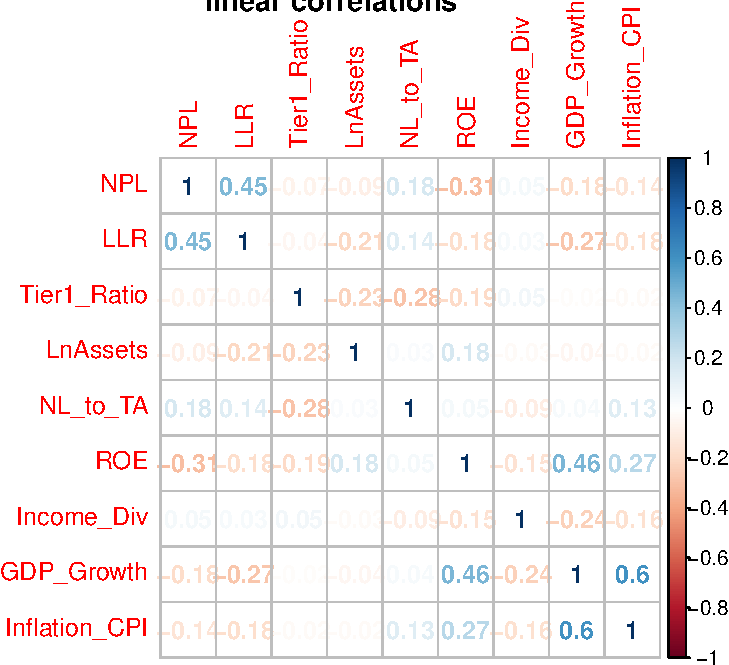
\includegraphics{preprint_files/figure-latex/correlation-1} \end{center}

Table 4 reports the Pearson correlation matrix between the predictor
variables. All correlation coefficients of the variables are lower than
0.6, except for the correlation between Tier 1 capital ratio and the
total capital ratio due to the different definition of capital ratios.
Therefore, the regression models will be run only using one of these two
capital ratios in one model, in order to avoid high collinearity.

\hypertarget{impact-on-bank-credit-risk-risk-based-capital-ratios}{%
\subsection{Impact on bank credit risk -- risk-based capital
ratios}\label{impact-on-bank-credit-risk-risk-based-capital-ratios}}

\begin{verbatim}
## 'data.frame':    2310 obs. of  17 variables:
##  $ Institution_Name: chr  "Agricultural Bank of China Ltd." "Anhui Lixin Rural Commercial Bank Co., Ltd" "Anhui Lujiang Rural Commercial Bank Co., Ltd" "Anhui Taihe Rural Commercial Bank Company Ltd." ...
##  $ Ownership       : Factor w/ 5 levels "Foreign Joint-stock",..: 5 3 3 3 3 2 2 4 3 1 ...
##  $ Type            : chr  "Big Six" "Rural commercial" "Rural commercial" "Rural commercial" ...
##  $ Listed          : chr  "Mainland" NA NA NA ...
##  $ Year            : Factor w/ 10 levels "2010","2011",..: 10 10 10 10 10 10 10 10 10 10 ...
##  $ NPL             : num  1.4 2.22 3.36 2.05 9.1 ...
##  $ LLR             : num  4.05 5.62 5.76 7.25 4.91 ...
##  $ Tier1_Ratio     : num  12.53 10.76 10.29 11.45 7.73 ...
##  $ TC_to_RWA       : num  16.13 14.63 13.48 13.39 9.13 ...
##  $ Total_Assets    : num  3.57e+09 2.65e+06 2.72e+06 2.79e+06 4.52e+06 ...
##  $ LnAssets        : num  22 14.8 14.8 14.8 15.3 ...
##  $ NL_to_TA        : num  51.5 49.9 49.1 57.4 63.7 ...
##  $ ROE             : num  11.81 20.87 6.86 12.44 5.72 ...
##  $ Income_Div      : num  0.347 0.824 0.492 0.072 0.335 ...
##  $ Concentration   : num  40.3 40.3 40.3 40.3 40.3 ...
##  $ GDP_Growth      : num  5.95 5.95 5.95 5.95 5.95 ...
##  $ Inflation_CPI   : num  2.9 2.9 2.9 2.9 2.9 ...
\end{verbatim}

\begin{verbatim}
## 
## % Table created by stargazer v.5.2.2 by Marek Hlavac, Harvard University. E-mail: hlavac at fas.harvard.edu
## % Date and time: Fri, Sep 10, 2021 - 17:43:15
## % Requires LaTeX packages: dcolumn 
## \begin{table}[!htbp] \centering 
##   \caption{Baseline Regression - Year Fixed Effect Model} 
##   \label{} 
## \begin{tabular}{@{\extracolsep{5pt}}lD{.}{.}{-3} D{.}{.}{-3} D{.}{.}{-3} D{.}{.}{-3} } 
## \\[-1.8ex]\hline 
## \hline \\[-1.8ex] 
##  & \multicolumn{4}{c}{\textit{Dependent variable:}} \\ 
## \cline{2-5} 
## \\[-1.8ex] & \multicolumn{2}{c}{NPL} & \multicolumn{2}{c}{LLR} \\ 
## \\[-1.8ex] & \multicolumn{1}{c}{(1)} & \multicolumn{1}{c}{(2)} & \multicolumn{1}{c}{(3)} & \multicolumn{1}{c}{(4)}\\ 
## \hline \\[-1.8ex] 
##  Tier1\_Ratio & -0.005^{***} &  & -0.003^{**} &  \\ 
##   & (0.001) &  & (0.001) &  \\ 
##   TC\_to\_RWA &  & -0.005^{***} &  & -0.003^{**} \\ 
##   &  & (0.001) &  & (0.001) \\ 
##   LnAssets & -0.051^{***} & -0.050^{***} & -0.187^{***} & -0.184^{***} \\ 
##   & (0.018) & (0.018) & (0.018) & (0.018) \\ 
##   NL\_to\_TA & 0.022^{***} & 0.023^{***} & 0.017^{***} & 0.018^{***} \\ 
##   & (0.003) & (0.003) & (0.003) & (0.003) \\ 
##   ROE & -0.054^{***} & -0.055^{***} & 0.024^{***} & 0.026^{***} \\ 
##   & (0.006) & (0.005) & (0.005) & (0.005) \\ 
##   Income\_Div & -0.003 & -0.00004 & -0.244^{***} & -0.240^{***} \\ 
##   & (0.075) & (0.075) & (0.072) & (0.071) \\ 
##   Concentration & -0.089 & -0.102^{*} & -0.083 & -0.091 \\ 
##   & (0.060) & (0.060) & (0.059) & (0.058) \\ 
##   GDP\_Growth & 0.137 & 0.153 & -0.195^{*} & -0.184^{*} \\ 
##   & (0.101) & (0.101) & (0.100) & (0.099) \\ 
##   Inflation\_CPI & 0.138 & 0.187 & 0.074 & 0.092 \\ 
##   & (0.261) & (0.262) & (0.257) & (0.255) \\ 
##   Constant & 4.401^{***} & 4.642^{***} & 10.153^{***} & 10.239^{***} \\ 
##   & (1.185) & (1.185) & (1.166) & (1.155) \\ 
##  \hline \\[-1.8ex] 
## Year Fixed Effects & \multicolumn{1}{c}{Yes} & \multicolumn{1}{c}{Yes} & \multicolumn{1}{c}{Yes} & \multicolumn{1}{c}{Yes} \\ 
## \hline \\[-1.8ex] 
## Observations & \multicolumn{1}{c}{1,621} & \multicolumn{1}{c}{1,649} & \multicolumn{1}{c}{1,817} & \multicolumn{1}{c}{1,847} \\ 
## R$^{2}$ & \multicolumn{1}{c}{0.157} & \multicolumn{1}{c}{0.163} & \multicolumn{1}{c}{0.175} & \multicolumn{1}{c}{0.180} \\ 
## Adjusted R$^{2}$ & \multicolumn{1}{c}{0.150} & \multicolumn{1}{c}{0.156} & \multicolumn{1}{c}{0.169} & \multicolumn{1}{c}{0.174} \\ 
## Residual Std. Error & \multicolumn{1}{c}{1.126 (df = 1606)} & \multicolumn{1}{c}{1.131 (df = 1634)} & \multicolumn{1}{c}{1.156 (df = 1802)} & \multicolumn{1}{c}{1.152 (df = 1832)} \\ 
## F Statistic & \multicolumn{1}{c}{21.376$^{***}$ (df = 14; 1606)} & \multicolumn{1}{c}{22.742$^{***}$ (df = 14; 1634)} & \multicolumn{1}{c}{27.382$^{***}$ (df = 14; 1802)} & \multicolumn{1}{c}{28.734$^{***}$ (df = 14; 1832)} \\ 
## \hline 
## \hline \\[-1.8ex] 
## \textit{Note:}  & \multicolumn{4}{r}{$^{*}$p$<$0.1; $^{**}$p$<$0.05; $^{***}$p$<$0.01} \\ 
## \end{tabular} 
## \end{table}
\end{verbatim}

Table 5 reports fixed effect baseline regression results for the full
sample of banks. The first two columns in Table 5 show regressions of
Non-Performing Loans to Gross Loans on regulatory capital requirements.
Columns (3) and (4) use Loan Loss Reserve to Gross Loans as the
dependent variable. We use a year fixed effect model here, in
consideration of that the effects of regulatory capital requirements
evolve through years and reducing the potential of omitted variables
{[}Zhang et al. (2016),RN19\}. Only one regulatory capital ratio is
employed as the variable of interest in each column. All four
regressions report negative and statistically significant relationships
between bank credit risk variables and risk-based capital ratios. The
results support the hypothesis: higher regulatory capital requirements
are related to lower bank credit risk.

The finding can be explained by the fact that those Chinese banks with
higher level of regulatory capital have higher capability to reduce the
impact of Non-Performing Loans, and thus lower Loan Loss Reserve. Tan
and Floros (2013) find a negative but insignificant relationship between
bank risk and capitalization when Loan Loss Reserve to Gross Loans is
employed as the proxy of risk. Lee, Ning, and Lee (2015) report a
significant negative relationship between bank capital and credit risk
(proxied by NPL ratio). This finding may reveal that the capital
adequacy requirements of Basel III equip commercial banks in China with
proper capital buffers in terms of mitigating credit risk.

Among bank-specific and macroeconomic control variables, we find that
LnAssets (a proxy of bank size), Net Loans to Total Assets (a proxy of
asset quality), and ROE (a proxy of profitability) are the most
significant variables. Bank size has a significant and negative impact
on Chinese banks' credit risk. This result is consistent with findings
from some studies regarding the impact of capital ratios on bank credit
risk {[}Tan and Floros (2013),RN28\}. This finding suggests that large
banks are more competent in dealing with risky loans and or they can
spread the risk across a larger more diverse loan risk profile. Because
large banks may benefit from firm reputation, compared to small banks,
and have wide-ranging access to fixed-income and equity markets to
diversify and hedge their credit risk. There is a significant and
negative relationship between banking industry concentration and
individual banks' credit risk. The total assets of the largest six
commercial banks\footnote{The largest six commercial banks: Industrial
  and Commercial Bank of China, Agricultural Bank of China, Bank of
  China, China Construction Bank, Bank of Communications, and Postal
  Savings Bank of China. The first four banks are listed as global
  systemically important banks (G-SIBs) in the FSB 2020 G-SIBs list.}
account for 41.87\% averagely during 2010-2019, although the industry
concentration shows roughly a year-by-year decrease in the past decade.
Four out of these six banks are listed as global systemically important
banks (G-SIBs) by FSB in 2020. In the context of China's banking
industry, these six banks have a better ability to reduce the pressure
in their credit activities, compared with other smaller-sized banks.

\hypertarget{impact-on-bank-credit-risk-ownership-structure}{%
\subsection{Impact on bank credit risk -- Ownership
structure}\label{impact-on-bank-credit-risk-ownership-structure}}

\begin{verbatim}
## 
## % Table created by stargazer v.5.2.2 by Marek Hlavac, Harvard University. E-mail: hlavac at fas.harvard.edu
## % Date and time: Fri, Sep 10, 2021 - 17:43:15
## % Requires LaTeX packages: dcolumn 
## \begin{table}[!htbp] \centering 
##   \caption{Fixed Effect Regression - Ownership Structure} 
##   \label{} 
## \begin{tabular}{@{\extracolsep{5pt}}lD{.}{.}{-3} D{.}{.}{-3} D{.}{.}{-3} D{.}{.}{-3} } 
## \\[-1.8ex]\hline 
## \hline \\[-1.8ex] 
##  & \multicolumn{4}{c}{\textit{Dependent variable:}} \\ 
## \cline{2-5} 
## \\[-1.8ex] & \multicolumn{2}{c}{NPL} & \multicolumn{2}{c}{LLR} \\ 
## \\[-1.8ex] & \multicolumn{1}{c}{(1)} & \multicolumn{1}{c}{(2)} & \multicolumn{1}{c}{(3)} & \multicolumn{1}{c}{(4)}\\ 
## \hline \\[-1.8ex] 
##  Tier1\_Ratio & -0.003^{**} &  & -0.0003 &  \\ 
##   & (0.001) &  & (0.001) &  \\ 
##   TC\_to\_RWA &  & -0.003^{**} &  & -0.0003 \\ 
##   &  & (0.001) &  & (0.001) \\ 
##   OwnershipForeign-owned & -0.858^{***} & -0.885^{***} & -1.555^{***} & -1.515^{***} \\ 
##   & (0.167) & (0.166) & (0.137) & (0.135) \\ 
##   OwnershipJoint-stock & 0.030 & 0.037 & -0.018 & -0.001 \\ 
##   & (0.115) & (0.115) & (0.110) & (0.109) \\ 
##   OwnershipLocal government-holding & 0.072 & 0.063 & -0.086 & -0.070 \\ 
##   & (0.118) & (0.118) & (0.113) & (0.112) \\ 
##   OwnershipState-owned & 0.123 & 0.119 & 0.077 & 0.082 \\ 
##   & (0.149) & (0.150) & (0.144) & (0.144) \\ 
##   LnAssets & -0.074^{***} & -0.073^{***} & -0.229^{***} & -0.225^{***} \\ 
##   & (0.023) & (0.023) & (0.021) & (0.021) \\ 
##   NL\_to\_TA & 0.019^{***} & 0.019^{***} & 0.010^{***} & 0.011^{***} \\ 
##   & (0.003) & (0.003) & (0.003) & (0.003) \\ 
##   ROE & -0.070^{***} & -0.071^{***} & -0.019^{***} & -0.016^{***} \\ 
##   & (0.006) & (0.006) & (0.005) & (0.005) \\ 
##   Income\_Div & 0.055 & 0.060 & -0.113^{*} & -0.110 \\ 
##   & (0.075) & (0.075) & (0.068) & (0.068) \\ 
##   Concentration & -0.088 & -0.100^{*} & -0.068 & -0.073 \\ 
##   & (0.059) & (0.059) & (0.055) & (0.055) \\ 
##   GDP\_Growth & 0.149 & 0.165^{*} & -0.157^{*} & -0.151 \\ 
##   & (0.100) & (0.100) & (0.094) & (0.093) \\ 
##   Inflation\_CPI & 0.161 & 0.211 & 0.043 & 0.053 \\ 
##   & (0.258) & (0.258) & (0.241) & (0.239) \\ 
##   Constant & 4.918^{***} & 5.173^{***} & 10.955^{***} & 10.978^{***} \\ 
##   & (1.218) & (1.218) & (1.131) & (1.122) \\ 
##  \hline \\[-1.8ex] 
## Year Fixed Effects & \multicolumn{1}{c}{Yes} & \multicolumn{1}{c}{Yes} & \multicolumn{1}{c}{Yes} & \multicolumn{1}{c}{Yes} \\ 
## \hline \\[-1.8ex] 
## Observations & \multicolumn{1}{c}{1,621} & \multicolumn{1}{c}{1,649} & \multicolumn{1}{c}{1,817} & \multicolumn{1}{c}{1,847} \\ 
## R$^{2}$ & \multicolumn{1}{c}{0.182} & \multicolumn{1}{c}{0.189} & \multicolumn{1}{c}{0.279} & \multicolumn{1}{c}{0.281} \\ 
## Adjusted R$^{2}$ & \multicolumn{1}{c}{0.173} & \multicolumn{1}{c}{0.180} & \multicolumn{1}{c}{0.272} & \multicolumn{1}{c}{0.274} \\ 
## Residual Std. Error & \multicolumn{1}{c}{1.111 (df = 1602)} & \multicolumn{1}{c}{1.115 (df = 1630)} & \multicolumn{1}{c}{1.082 (df = 1798)} & \multicolumn{1}{c}{1.080 (df = 1828)} \\ 
## F Statistic & \multicolumn{1}{c}{19.794$^{***}$ (df = 18; 1602)} & \multicolumn{1}{c}{21.099$^{***}$ (df = 18; 1630)} & \multicolumn{1}{c}{38.703$^{***}$ (df = 18; 1798)} & \multicolumn{1}{c}{39.691$^{***}$ (df = 18; 1828)} \\ 
## \hline 
## \hline \\[-1.8ex] 
## \textit{Note:}  & \multicolumn{4}{r}{$^{*}$p$<$0.1; $^{**}$p$<$0.05; $^{***}$p$<$0.01} \\ 
## \end{tabular} 
## \end{table}
\end{verbatim}

Table 6 reports the results of the impact on bank credit risk by adding
banks' ownership structure as a specific control variable. We find that
adding ownership structure does not change the significant and negative
impact of bank size, net loans to total assets and industry
concentration on bank credit risk, respectively. However, the
relationship between capital requirements and Loan Loss Reserve ratio
has become insignificant, although it remains negative. The regressions
presented in Table 6 demonstrate that ownership structure is positively
associated with bank credit risk. This finding is consistent with the
view that shareholders have greater incentives for risky projects than
managers (John, Litov, and Yeung 2008). This finding also supports the
empirical results of Laeven and Levine (2009){]} where they find a
positive association between risk and ownership of a large owner (10\%
or more voting rights).

As discussed in the previous sections, ownership structure is always one
of the focusing areas of research on China's banking industry. Berger,
Hasan, and Zhou (2009)\} studies efficiency of Chinese banks from the
perspective of ownership structure and suggests that minority of foreign
ownership helps improve bank efficiency. Pessarossi and Weill (2015)\}
investigates the effect of capital ratio on Chinese banks' cost
efficiency adjusting for ownership structure. Zhang et al. (2016)\}
compares bank risks between different ownership structures of Chinese
banks. The reason that the ownership structure becomes of one of the
main interest factors in Chinese banking research could stem from the
unique growth path of China's banking industry and the suspicious in
Western democracies of latent state manipulation. The past four decades
witnessed dramatic changes and development in China's banking sector.
The three stages of the reform in China's banking industry achieves the
advancement of the legal and financial infrastructure, as well as the
more diversified ownership structure. By 2010 the four G-SIBs and other
12 commercial banks all finished IPOs. Private shareholding accounted
for 77.7\% in rural commercial banks. The period after 2010 could be
considered not only as a stage of the financial reform for further
progressing and improving, but also a time to evaluate the effectiveness
of the substantial bank ownership changes. In recent times, as China
seeks to decouple its reserve banking system from the US, there may be
important implications for continued regulatory cooperation in
international banking\footnote{\url{https://rhg.com/research/us-china-decoupling}}

The results reveal that state-owned banks have higher credit risk
compared to those foreign-owned banks in China's banking industry. This
finding, to some extent, supports the viewpoint that state-owned banks
would be involved in policy-guided credit activities instead of
profit-centered ones (Pessarossi and Weill 2015). The social lending
theory of state ownership Atkinson (1980) suggests that state-owned
enterprises contribute to ``correcting the `failure' of market economy''
due to imperfect competition, inefficiency and public good. According to
this view, government-owned enterprises may help improve the overall
economy performance (Stiglitz 1993). In China's banking context, the
biggest four commercial banks were founded and conducted a large amount
of government lending in the early 1990's, before national banks and
city banks were established. Within a relatively long period, the
state-owned banks (including local government-holding banks founded
later in the end of 1990's) played a role of `government agencies' to
pursue the broader social welfare objectives rather than profit
maximizing. Since the state-owned banks target multiple welfare
objectives which might not be measurable, the managers in the
state-owned banks have low powered incentives(Tirole 1994). However,
this resulted in the significant non-performing loan levels of `Big
Four' banks before China's WTO accession in 2001.

Since 2001, the ownership structure has been dramatically transformed,
due to China's overall industrial reforms and the commitments to the WTO
agreement. The large part of shares directly held by local government
were gradually replaced by mixed ownership enterprises, foreign
investments, and private investors. In terms of the state-owned banks,
direct state intervention was replaced by Central Huijin (a company
representing the state government) along with the establishment of
modern corporate governance system. Why does state ownership still have
relatively higher credit risk? The higher credit risk taking by
state-owned banks can be explained by two reasons: (1) although the
direct government shareholding structure changed, business connection
with state-owned enterprises remains due to the long-lasting business
relationship and contracts such as those nationwide infrastructure
projects lasting for decades; (2) the development of modern corporate
governance mechanisms in China's banking industry could transform
government ownership into concentrated ownership, the ownership similar
to the one of large investors with significant control rights and cash
flow rights {[}Shleifer and Vishny (1997)\}. From this perspective,
concentrated ownership puts pressure on management decision {[}Shleifer
and Vishny (1997)\} and bank risk taking incentives {[}Boyd and Hakenes
(2008)\} Almost all state-owned banks are listed banks. With their
significant control rights and cash flow rights, the state (large)
shareholder in these state-owned, listed banks may take excessive risk
by favouring particular clientele such as large conglomerates in
projects with potential of social-benefits rather than those with target
of profit-maximizing. Sapienza (2004)\} finds that state-owned banks
favour large firms and charge lower interest rates than other types of
banks in Italy. This finding is also consistent with Laeven and Levine
(2009)\} where they report banks with large investors have higher risk.

\hypertarget{impact-on-bank-credit-risk-interaction-between-regulation-and-ownership-structure}{%
\subsection{Impact on bank credit risk -- Interaction between regulation
and ownership
structure\}}\label{impact-on-bank-credit-risk-interaction-between-regulation-and-ownership-structure}}

\begin{verbatim}
## 
## % Table created by stargazer v.5.2.2 by Marek Hlavac, Harvard University. E-mail: hlavac at fas.harvard.edu
## % Date and time: Fri, Sep 10, 2021 - 17:43:16
## % Requires LaTeX packages: dcolumn 
## \begin{table}[!htbp] \centering 
##   \caption{Table 7: Regression with Interaction between Ownership and Regulation} 
##   \label{} 
## \begin{tabular}{@{\extracolsep{5pt}}lD{.}{.}{-3} D{.}{.}{-3} D{.}{.}{-3} D{.}{.}{-3} } 
## \\[-1.8ex]\hline 
## \hline \\[-1.8ex] 
##  & \multicolumn{4}{c}{\textit{Dependent variable:}} \\ 
## \cline{2-5} 
## \\[-1.8ex] & \multicolumn{2}{c}{NPL} & \multicolumn{2}{c}{LLR} \\ 
## \\[-1.8ex] & \multicolumn{1}{c}{(1)} & \multicolumn{1}{c}{(2)} & \multicolumn{1}{c}{(3)} & \multicolumn{1}{c}{(4)}\\ 
## \hline \\[-1.8ex] 
##  Tier1\_Ratio & -0.078 &  & -0.049^{***} &  \\ 
##   & (0.072) &  & (0.013) &  \\ 
##   TC\_to\_RWA &  & -0.040 &  & -0.039^{***} \\ 
##   &  & (0.065) &  & (0.009) \\ 
##   OwnershipForeign-owned & -1.747^{**} & -1.456^{*} & -2.126^{***} & -2.119^{***} \\ 
##   & (0.767) & (0.857) & (0.211) & (0.198) \\ 
##   OwnershipJoint-stock & -0.018 & 0.860 & -0.804^{***} & -0.819^{***} \\ 
##   & (0.763) & (0.866) & (0.240) & (0.256) \\ 
##   OwnershipLocal government-holding & 0.235 & 0.585 & -0.951^{***} & -1.215^{***} \\ 
##   & (0.794) & (0.908) & (0.317) & (0.364) \\ 
##   OwnershipState-owned & 0.227 & 0.913 & -0.015 & -0.374 \\ 
##   & (0.897) & (1.069) & (0.522) & (0.670) \\ 
##   LnAssets & -0.106^{***} & -0.100^{***} & -0.229^{***} & -0.229^{***} \\ 
##   & (0.023) & (0.023) & (0.022) & (0.022) \\ 
##   NL\_to\_TA & 0.018^{***} & 0.019^{***} & 0.010^{***} & 0.010^{***} \\ 
##   & (0.003) & (0.003) & (0.003) & (0.003) \\ 
##   ROE & -0.074^{***} & -0.072^{***} & -0.020^{***} & -0.018^{***} \\ 
##   & (0.006) & (0.006) & (0.005) & (0.005) \\ 
##   Income\_Div & 0.020 & 0.022 & -0.104 & -0.094 \\ 
##   & (0.074) & (0.074) & (0.068) & (0.068) \\ 
##   Concentration & -0.095 & -0.108^{*} & -0.065 & -0.070 \\ 
##   & (0.058) & (0.058) & (0.055) & (0.054) \\ 
##   GDP\_Growth & 0.165^{*} & 0.164^{*} & -0.163^{*} & -0.154^{*} \\ 
##   & (0.099) & (0.098) & (0.093) & (0.092) \\ 
##   Inflation\_CPI & 0.228 & 0.267 & 0.027 & 0.034 \\ 
##   & (0.256) & (0.254) & (0.240) & (0.238) \\ 
##   Tier1\_Ratio:OwnershipForeign-owned & 0.075 &  & 0.049^{***} &  \\ 
##   & (0.072) &  & (0.013) &  \\ 
##   Tier1\_Ratio:OwnershipJoint-stock & 0.009 &  & 0.069^{***} &  \\ 
##   & (0.073) &  & (0.019) &  \\ 
##   Tier1\_Ratio:OwnershipLocal government-holding & -0.013 &  & 0.077^{***} &  \\ 
##   & (0.076) &  & (0.027) &  \\ 
##   Tier1\_Ratio:OwnershipState-owned & -0.001 &  & 0.006 &  \\ 
##   & (0.085) &  & (0.047) &  \\ 
##   TC\_to\_RWA:OwnershipForeign-owned &  & 0.038 &  & 0.039^{***} \\ 
##   &  & (0.065) &  & (0.009) \\ 
##   TC\_to\_RWA:OwnershipJoint-stock &  & -0.061 &  & 0.057^{***} \\ 
##   &  & (0.067) &  & (0.017) \\ 
##   TC\_to\_RWA:OwnershipLocal government-holding &  & -0.041 &  & 0.083^{***} \\ 
##   &  & (0.070) &  & (0.026) \\ 
##   TC\_to\_RWA:OwnershipState-owned &  & -0.057 &  & 0.032 \\ 
##   &  & (0.082) &  & (0.051) \\ 
##   Constant & 6.379^{***} & 6.351^{***} & 11.526^{***} & 11.584^{***} \\ 
##   & (1.430) & (1.482) & (1.148) & (1.135) \\ 
##  \hline \\[-1.8ex] 
## Year Fixed Effects & \multicolumn{1}{c}{Yes} & \multicolumn{1}{c}{Yes} & \multicolumn{1}{c}{Yes} & \multicolumn{1}{c}{Yes} \\ 
## \hline \\[-1.8ex] 
## Observations & \multicolumn{1}{c}{1,621} & \multicolumn{1}{c}{1,649} & \multicolumn{1}{c}{1,817} & \multicolumn{1}{c}{1,847} \\ 
## R$^{2}$ & \multicolumn{1}{c}{0.199} & \multicolumn{1}{c}{0.216} & \multicolumn{1}{c}{0.287} & \multicolumn{1}{c}{0.290} \\ 
## Adjusted R$^{2}$ & \multicolumn{1}{c}{0.188} & \multicolumn{1}{c}{0.205} & \multicolumn{1}{c}{0.278} & \multicolumn{1}{c}{0.281} \\ 
## Residual Std. Error & \multicolumn{1}{c}{1.100 (df = 1598)} & \multicolumn{1}{c}{1.098 (df = 1626)} & \multicolumn{1}{c}{1.078 (df = 1794)} & \multicolumn{1}{c}{1.074 (df = 1824)} \\ 
## F Statistic & \multicolumn{1}{c}{18.102$^{***}$ (df = 22; 1598)} & \multicolumn{1}{c}{20.305$^{***}$ (df = 22; 1626)} & \multicolumn{1}{c}{32.750$^{***}$ (df = 22; 1794)} & \multicolumn{1}{c}{33.874$^{***}$ (df = 22; 1824)} \\ 
## \hline 
## \hline \\[-1.8ex] 
## \textit{Note:}  & \multicolumn{4}{r}{$^{*}$p$<$0.1; $^{**}$p$<$0.05; $^{***}$p$<$0.01} \\ 
## \end{tabular} 
## \end{table}
\end{verbatim}

Table 7 presents regressions in which we assess the interactive
associations among ownership structure, regulatory capital requirements,
and bank credit risk. Some studies suggest that the relationship between
risk and ownership structure is closely associated with national
regulation. Because regulation influences both bank owners' and bank
managers' incentives of risk-taking and risk-shifting {[}John, Saunders,
and Senbet (2000);RN54{]}. Laeven and Levine (2009) examine the
interactions between ownership structure and national regulatory
requirements and stringency, and find the relationship between risk and
regulation stringency depends on ownership structure. Berger and Bouwman
(2013) state that capital requirements have different impact on bank
performance based on different bank size. Here we include the
interaction term of each of the capital adequacy variables with
different ownership structure variables. Capital adequacy variables
remain negative but become insignificant, except for Tier 1 Ratio
remains significant but lowers its significant level, under the
circumstance of the interactive association between capital ratios and
ownership structure. This finding demonstrates the direct effect of the
capital adequacy requirement is to reduce bank credit risk and to
enhance bank stability.

After add in the interactive term, the coefficients of the ownership
structure variables show positively and significantly in Table 7. This
finding may partially support the theories arguing that bank owners may
choose to increase portfolio risk when facing more stringent capital
requirements, in order to compensate their potential loss of expected
utility {[}Koehn and Santomero (1980);RN34{]}. Table 7 shows that local
government-holding banks have a higher positive coefficient than other
types of banks, indicating that local government-holding banks may have
higher incentives to reshuffle risk when facing higher capital adequacy
regulation.

In regression (1) that include the interaction term between capital
ratio and ownership structure, the coefficient of Tie 1 Ratio stays
negative and statistically significant. This result reveals that the
effect of capital regulation is to mitigate bank credit risk and enhance
bank stability, which is also in accordance with banking regulation
theories. This result may also indicate that the impact of capital
regulation on credit risk, to some extent, depends on ownership
structure. The interactive coefficient estimates for Tier 1
Ratio*different ownership structure are negative. Among these terms, the
joint-stock and local government-holding terms enter significantly. This
shows that the impact on bank credit risk of Tier 1 ratio can be
magnified when banks are not dominated by a single large owner\footnote{In
  our sample, the direct(indirect) shares of local government-holding
  banks held by government or its agencies are over 10\%. However, the
  local government-holding banks don't have dominant direct(indirect)
  government shareholders (50\% more voting rights). In fact, most of
  these banks are widely held and have mixed-ownership shareholders.}.
However, Tier 1 Ratio does not have significant non-linear impact on
bank credit risk when banks are state-owned. Laeven and Levine (2009)
argue that regulations affecting risk-taking incentives of banks with
powerful owners and the ones widely held may be in different ways. The
finding may be interpreted that the interaction between capital
regulations and the incentives of joint-stock shareholders is more
significant than powerful shareholders, because shareholders of
joint-stock banks may have different risk-taking incentives from the
influential state-shareholders. This result also collaborates with the
estimates of the coefficients of ownership structure.

\hypertarget{conclusion}{%
\section{Conclusion}\label{conclusion}}

This paper aims to analyze the impact of capital regulation on Chinese
banks' credit risk-taking following the 2007-2009 global financial
crisis and to assess the impact of capital regulation on credit
risk-taking by incorporating the interaction between capital regulation
and ownership structure. We focus on risk-based capital regulation from
the Basel III framework that affects Chinese commercial banks over the
period 2010-2019. This period coincides with the fourth stage of China's
financial reform and the implementation of Basel III framework in China.
Financial theories, supported by empirical studies, suggest that the
impact of bank regulation on bank risk-taking varies due to different
ownership structure \{RN1\}. Therefore, this study provides implications
for regulatory strategies and the stability of China's banking system.

We find that Basel III risk-based capital regulation has a negative
impact on bank credit risk-taking. This finding implies that
implementation of Basel III capital regulation has strengthened
financial stability. We compare the credit risk-taking level of
different ownership structure in China's commercial banks and find that
state-owned banks have higher credit risk-taking than any other
ownership structure in China's banking industry. This finding is
consistent with the social view of the state ownership theory, as well
as the theory predicting that powerful shareholders have stronger
incentives to take risks due to the transformation of ownership
structure during China's financial reform.

Furthermore, we find that the impact of capital regulation on credit
risk-taking is influenced by ownership structure. The same bank
regulations have different effects on credit risk-taking because of the
interaction between bank regulation and ownership structure. Thus, this
paper provides strategic implication for regulatory authorities making
regulatory decisions to take into account bank ownership structure.

\hypertarget{appendix}{%
\section{Appendix}\label{appendix}}

\hypertarget{a1.-definitions-of-the-basel-accords}{%
\subsection{A1. Definitions of the Basel
Accords}\label{a1.-definitions-of-the-basel-accords}}

\hypertarget{references}{%
\section*{References}\label{references}}
\addcontentsline{toc}{section}{References}

\hypertarget{refs}{}
\leavevmode\hypertarget{ref-RN15}{}%
Allen, Franklin, Elena Carletti, and Robert Marquez. 2011. ``Credit
Market Competition and Capital Regulation.'' Journal Article. \emph{The
Review of Financial Studies} 24 (4): 983--1018.
\url{http://www.jstor.org.queens.ezp1.qub.ac.uk/stable/20869263}.

\leavevmode\hypertarget{ref-RN16}{}%
Amihud, Yakov, and Baruch Lev. 1981. ``Risk Reduction as a Managerial
Motive for Conglomerate Mergers.'' Journal Article. \emph{The Bell
Journal of Economics} 12 (2): 605--17.
\url{https://doi.org/10.2307/3003575}.

\leavevmode\hypertarget{ref-RN17}{}%
Andrianova, Svetlana, Panicos Demetriades, and Anja Shortland. 2012.
``Government Ownership of Banks, Institutions and Economic Growth.''
Journal Article. \emph{Economica} 79 (315): 449--69.
\url{http://www.jstor.org/stable/23274805}.

\leavevmode\hypertarget{ref-RN18}{}%
Anginer, Deniz, and Asli Demirguc-Kunt. 2014. ``Bank Capital and
Systemic Stability.'' Journal Article. \emph{Policy Research Working
Papers} 6948 (June 2014): 42.
\url{https://doi.org/doi:10.1596/1813-9450-6948}.

\leavevmode\hypertarget{ref-RN20}{}%
Atkinson, Joseph. E., Anthony. B.; Stiglitz. 1980. \emph{Lectures on
Public Economics}. Book. London ; New York: McGraw-Hill Book Co.

\leavevmode\hypertarget{ref-RN21}{}%
Ayadi, Rym, Paola Bongini, Barbara Casu, and Doriana Cucinelli. 2020.
``Bank Business Model Migrations in Europe: Determinants and Effects.''
Journal Article. \emph{British Journal of Management} n/a (n/a).
\url{https://doi.org/https://doi.org/10.1111/1467-8551.12437}.

\leavevmode\hypertarget{ref-RN22}{}%
Beck, Thorsten, Asli Demirgüç-Kunt, and Vojislav Maksimovic. 2004.
``Bank Competition and Access to Finance: International Evidence.''
Journal Article. \emph{Journal of Money, Credit and Banking} 36 (3):
627--48.
\url{http://www.jstor.org.queens.ezp1.qub.ac.uk/stable/3838958}.

\leavevmode\hypertarget{ref-RN23}{}%
Beck, Thorsten, and Ross Levine. 2002. ``Industry Growth and Capital
Allocation:: Does Having a Market- or Bank-Based System Matter?''
Journal Article. \emph{Journal of Financial Economics} 64 (2): 147--80.
\url{https://doi.org/https://doi.org/10.1016/S0304-405X(02)00074-0}.

\leavevmode\hypertarget{ref-RN24}{}%
Berger, Allen N., and Christa H. S. Bouwman. 2013. ``How Does Capital
Affect Bank Performance During Financial Crises?'' Journal Article.
\emph{Journal of Financial Economics} 109 (1): 146--76.
\url{https://doi.org/https://doi.org/10.1016/j.jfineco.2013.02.008}.

\leavevmode\hypertarget{ref-RN25}{}%
Berger, Allen N., George R. G. Clarke, Robert Cull, Leora Klapper, and
Gregory F. Udell. 2005. ``Corporate Governance and Bank Performance: A
Joint Analysis of the Static, Selection, and Dynamic Effects of
Domestic, Foreign, and State Ownership.'' Journal Article. \emph{Journal
of Banking \& Finance} 29 (8): 2179--2221.
\url{https://doi.org/https://doi.org/10.1016/j.jbankfin.2005.03.013}.

\leavevmode\hypertarget{ref-RN26}{}%
Berger, Allen N., Iftekhar Hasan, and Mingming Zhou. 2009. ``Bank
Ownership and Efficiency in China: What Will Happen in the World's
Largest Nation?'' Journal Article. \emph{Journal of Banking \& Finance}
33 (1): 113--30.
\url{https://doi.org/https://doi.org/10.1016/j.jbankfin.2007.05.016}.

\leavevmode\hypertarget{ref-RN28}{}%
Bitar, Mohammad, Kuntara Pukthuanthong, and Thomas Walker. 2018. ``The
Effect of Capital Ratios on the Risk, Efficiency and Profitability of
Banks: Evidence from Oecd Countries.'' Journal Article. \emph{Journal of
International Financial Markets, Institutions and Money} 53: 227--62.
\url{https://doi.org/https://doi.org/10.1016/j.intfin.2017.12.002}.

\leavevmode\hypertarget{ref-RN29}{}%
Blum, Jürg. 1999. ``Do Capital Adequacy Requirements Reduce Risks in
Banking?'' Journal Article. \emph{Journal of Banking \& Finance} 23 (5):
755--71.
\url{https://doi.org/https://doi.org/10.1016/S0378-4266(98)00113-7}.

\leavevmode\hypertarget{ref-RN30}{}%
Borio, Claudio. E. V. 2003. ``Towards a Macroprudential Framework for
Financial Supervision and Regulation?'' Journal Article. \emph{BIS
Working Papers} no. 128. (Accessed from
https://nla.gov.au/nla.cat-vn1001461): 1020--0959.

\leavevmode\hypertarget{ref-RN32}{}%
Boyd, John H., and Gianni De Nicoló. 2005. ``The Theory of Bank Risk
Taking and Competition Revisited.'' Journal Article. \emph{The Journal
of Finance} 60 (3): 1329--43.
\url{http://www.jstor.org.queens.ezp1.qub.ac.uk/stable/3694928}.

\leavevmode\hypertarget{ref-RN31}{}%
Boyd, John H., and Hendrik Hakenes. 2008. ``Looting and Gambling in
Banking Crises.'' Conference Proceedings. In.

\leavevmode\hypertarget{ref-RN33}{}%
Burkart, Mike, Fausto Panunzi, and Andrei Shleifer. 2003. ``Family
Firms.'' Journal Article. \emph{The Journal of Finance} 58 (5):
2167--2201.
\url{https://doi.org/https://doi.org/10.1111/1540-6261.00601}.

\leavevmode\hypertarget{ref-RN35}{}%
Calem, Paul, and Rafael Rob. 1999. ``The Impact of Capital-Based
Regulation on Bank Risk-Taking.'' Journal Article. \emph{Journal of
Financial Intermediation} 8 (4): 317--52.
\url{https://doi.org/https://doi.org/10.1006/jfin.1999.0276}.

\leavevmode\hypertarget{ref-RN36}{}%
Chiaramonte, Laura, and Barbara Casu. 2017. ``Capital and Liquidity
Ratios and Financial Distress. Evidence from the European Banking
Industry.'' Journal Article. \emph{The British Accounting Review} 49
(2): 138--61.
\url{https://doi.org/https://doi.org/10.1016/j.bar.2016.04.001}.

\leavevmode\hypertarget{ref-RN37}{}%
Cooper, Russell, and Thomas W. Ross. 2002. ``Bank Runs: Deposit
Insurance and Capital Requirements.'' \emph{International Economic
Review} 43 (1): 55--72.
\url{http://www.jstor.org.queens.ezp1.qub.ac.uk/stable/827056}.

\leavevmode\hypertarget{ref-RN40}{}%
Dagher, Jihad, Giovanni Dell'Ariccia, Luc Laeven, Lev Ratnovski, and Hui
Tong. 2016. ``Benefits and Costs of Bank Capital.'' Journal Article.
\emph{Staff Discussion Notes} 2016 (004): A001.
\url{https://doi.org/10.5089/9781498387712.006.A001}.

\leavevmode\hypertarget{ref-RN41}{}%
Demirguc-Kunt, Asli; and Enrica Detragiache. 1997. ``The Determinants of
Banking Crises : Evidence from Industrial and Developing Countries.''
Journal Article. \emph{Policy Research Working Papers}, nos. Accessed
from https://nla.gov.au/nla.cat-vn679349.

\leavevmode\hypertarget{ref-RN42}{}%
Demirguc-Kunt, Asli, Enrica Detragiache, and Ouarda Merrouche. 2013.
``Bank Capital: Lessons from the Financial Crisis.'' Journal Article.
\emph{Journal of Money, Credit and Banking} 45 (6): 1147--64.
\url{http://www.jstor.org.queens.ezp1.qub.ac.uk/stable/23463595}.

\leavevmode\hypertarget{ref-RN43}{}%
Demirgüç-Kunt, Asli, and Harry Huizinga. 2010. ``Bank Activity and
Funding Strategies: The Impact on Risk and Returns.'' Journal Article.
\emph{Journal of Financial Economics} 98 (3): 626--50.
\url{https://doi.org/https://doi.org/10.1016/j.jfineco.2010.06.004}.

\leavevmode\hypertarget{ref-RN44}{}%
Demirgüç-Kunt, Asli, and Edward J. Kane. 2002. ``Deposit Insurance
Around the Globe: Where Does It Work?'' Journal Article. \emph{The
Journal of Economic Perspectives} 16 (2): 175--95.
\url{http://www.jstor.org.queens.ezp1.qub.ac.uk/stable/2696502}.

\leavevmode\hypertarget{ref-RN45}{}%
Diamond, Douglas W. 1984. ``Financial Intermediation and Delegated
Monitoring.'' Journal Article. \emph{Review of Economic Studies} 51 (3):
393. \url{https://doi.org/10.2307/2297430}.

\leavevmode\hypertarget{ref-RN46}{}%
Diamond, Douglas W., and Philip H. Dybvig. 1983. ``Bank Runs, Deposit
Insurance, and Liquidity.'' Journal Article. \emph{Journal of Political
Economy} 91 (3): 401--19. \url{http://www.jstor.org/stable/1837095}.

\leavevmode\hypertarget{ref-RN47}{}%
Fungáčová, Zuzana, Pierre Pessarossi, and Laurent Weill. 2013. ``Is Bank
Competition Detrimental to Efficiency? Evidence from China.'' Journal
Article. \emph{China Economic Review} 27: 121--34.
\url{https://doi.org/https://doi.org/10.1016/j.chieco.2013.09.004}.

\leavevmode\hypertarget{ref-RN48}{}%
Hellmann, Thomas F., Kevin C. Murdock, and Joseph E. Stiglitz. 2000.
``Liberalization, Moral Hazard in Banking, and Prudential Regulation:
Are Capital Requirements Enough?'' Journal Article. \emph{The American
Economic Review} 90 (1): 147--65.
\url{http://www.jstor.org.queens.ezp1.qub.ac.uk/stable/117285}.

\leavevmode\hypertarget{ref-RN49}{}%
Hirshleifer, David, and Anjan V. Thakor. 1992. ``Managerial
Conservatism, Project Choice, and Debt.'' Journal Article. \emph{The
Review of Financial Studies} 5 (3): 437--70.
\url{http://www.jstor.org.queens.ezp1.qub.ac.uk/stable/2962134}.

\leavevmode\hypertarget{ref-RN50}{}%
Hogan, Thomas L. 2015. ``Capital and Risk in Commercial Banking: A
Comparison of Capital and Risk-Based Capital Ratios.'' Journal Article.
\emph{The Quarterly Review of Economics and Finance} 57: 32--45.
\url{https://doi.org/https://doi.org/10.1016/j.qref.2014.11.003}.

\leavevmode\hypertarget{ref-RN51}{}%
Iannotta, Giuliano, Giacomo Nocera, and Andrea Sironi. 2007. ``Ownership
Structure, Risk and Performance in the European Banking Industry.''
Journal Article. \emph{Journal of Banking \& Finance} 31 (7): 2127--49.
\url{https://doi.org/https://doi.org/10.1016/j.jbankfin.2006.07.013}.

\leavevmode\hypertarget{ref-RN52}{}%
Jensen, Michael C., and William H. Meckling. 1976. ``Theory of the Firm:
Managerial Behavior, Agency Costs and Ownership Structure.'' Journal
Article. \emph{Journal of Financial Economics} 3 (4): 305--60.
\url{https://doi.org/https://doi.org/10.1016/0304-405X(76)90026-X}.

\leavevmode\hypertarget{ref-RN53}{}%
Jiang, Hai, Jinyi Zhang, and Chen Sun. 2020. ``How Does Capital Buffer
Affect Bank Risk-Taking? New Evidence from China Using Quantile
Regression.'' Journal Article. \emph{China Economic Review} 60: 101300.
\url{https://doi.org/https://doi.org/10.1016/j.chieco.2019.04.008}.

\leavevmode\hypertarget{ref-RN54}{}%
John, Kose, Lubomir Litov, and Bernard Yeung. 2008. ``Corporate
Governance and Risk-Taking.'' Journal Article. \emph{The Journal of
Finance} 63 (4): 1679--1728.
\url{http://www.jstor.org.queens.ezp1.qub.ac.uk/stable/25094487}.

\leavevmode\hypertarget{ref-RN55}{}%
John, Kose, Anthony Saunders, and Lemma W. Senbet. 2000. ``A Theory of
Bank Regulation and Management Compensation.'' Journal Article.
\emph{The Review of Financial Studies} 13 (1): 95--125.
\url{http://www.jstor.org.queens.ezp1.qub.ac.uk/stable/2646082}.

\leavevmode\hypertarget{ref-RN56}{}%
Keeley, Michael C. 1990. ``Deposit Insurance, Risk, and Market Power in
Banking.'' Journal Article. \emph{The American Economic Review} 80 (5):
1183--1200.
\url{http://www.jstor.org.queens.ezp1.qub.ac.uk/stable/2006769}.

\leavevmode\hypertarget{ref-RN57}{}%
Koehn, Michael, and Anthony M. Santomero. 1980. ``Regulation of Bank
Capital and Portfolio Risk.'' Journal Article. \emph{The Journal of
Finance} 35 (5): 1235--44. \url{https://doi.org/10.2307/2327096}.

\leavevmode\hypertarget{ref-RN60}{}%
Laeven, Luc, and Ross Levine. 2007. ``Is There a Diversification
Discount in Financial Conglomerates?'' Journal Article. \emph{Journal of
Financial Economics} 85 (2): 331--67.
\url{https://doi.org/https://doi.org/10.1016/j.jfineco.2005.06.001}.

\leavevmode\hypertarget{ref-RN1}{}%
---------. 2009. ``Bank Governance, Regulation and Risk Taking.''
Journal Article. \emph{Journal of Financial Economics} 93 (2): 259--75.
\url{https://doi.org/https://doi.org/10.1016/j.jfineco.2008.09.003}.

\leavevmode\hypertarget{ref-RN58}{}%
La Porta, Rafael, Lopez-de-Silanes Florencio, and Andrei Shleifer. 1999.
``Corporate Ownership Around the World.'' Journal Article. \emph{The
Journal of Finance} 54 (2): 471--517.
\url{http://www.jstor.org.queens.ezp1.qub.ac.uk/stable/2697717}.

\leavevmode\hypertarget{ref-RN59}{}%
---------. 2002. ``Government Ownership of Banks.'' Journal Article.
\emph{The Journal of Finance} 57 (1): 265--301.
\url{http://www.jstor.org.queens.ezp1.qub.ac.uk/stable/2697840}.

\leavevmode\hypertarget{ref-RN61}{}%
Lee, Chien-Chiang, and Meng-Fen Hsieh. 2013. ``The Impact of Bank
Capital on Profitability and Risk in Asian Banking.'' Journal Article.
\emph{Journal of International Money and Finance} 32: 251--81.
\url{https://doi.org/https://doi.org/10.1016/j.jimonfin.2012.04.013}.

\leavevmode\hypertarget{ref-RN62}{}%
Lee, Chien-Chiang, Shao-Lin Ning, and Chi-Chuan Lee. 2015. ``How Does
Bank Capital Affect Bank Profitability and Risk? Evidence from China's
Wto Accession.'' Journal Article. \emph{China \& World Economy} 23 (4):
19--39. \url{https://doi.org/https://doi.org/10.1111/cwe.12119}.

\leavevmode\hypertarget{ref-RN63}{}%
Lee, Tung-Hao, and Shu-Hwa Chih. 2013. ``Does Financial Regulation
Affect the Profit Efficiency and Risk of Banks? Evidence from China's
Commercial Banks.'' Journal Article. \emph{The North American Journal of
Economics and Finance} 26: 705--24.
\url{https://doi.org/https://doi.org/10.1016/j.najef.2013.05.005}.

\leavevmode\hypertarget{ref-RN64}{}%
Mehran, Hamid, and Anjan Thakor. 2011. ``Bank Capital and Value in the
Cross-Section.'' Journal Article. \emph{The Review of Financial Studies}
24 (4): 1019--67.
\url{http://www.jstor.org.queens.ezp1.qub.ac.uk/stable/20869264}.

\leavevmode\hypertarget{ref-RN65}{}%
Pasiouras, Fotios. 2008. ``International Evidence on the Impact of
Regulations and Supervision on Banks' Technical Efficiency: An
Application of Two-Stage Data Envelopment Analysis.'' Journal Article.
\emph{Review of Quantitative Finance and Accounting} 30 (2): 187--223.
\url{https://doi.org/10.1007/s11156-007-0046-7}.

\leavevmode\hypertarget{ref-RN66}{}%
Pessarossi, Pierre, and Laurent Weill. 2015. ``Do Capital Requirements
Affect Cost Efficiency? Evidence from China.'' Journal Article.
\emph{Journal of Financial Stability} 19: 119--27.
\url{https://doi.org/https://doi.org/10.1016/j.jfs.2014.11.002}.

\leavevmode\hypertarget{ref-RN68}{}%
Roulet, Caroline. 2018. ``Basel Iii: Effects of Capital and Liquidity
Regulations on European Bank Lending.'' Journal Article. \emph{Journal
of Economics and Business} 95: 26--46.
\url{https://doi.org/https://doi.org/10.1016/j.jeconbus.2017.10.001}.

\leavevmode\hypertarget{ref-RN69}{}%
Sapienza, Paola. 2004. ``The Effects of Government Ownership on Bank
Lending.'' Journal Article. \emph{Journal of Financial Economics} 72
(2): 357--84.
\url{https://doi.org/https://doi.org/10.1016/j.jfineco.2002.10.002}.

\leavevmode\hypertarget{ref-RN70}{}%
Saunders, Anthony, Elizabeth Strock, and Nickolaos G. Travlos. 1990.
``Ownership Structure, Deregulation, and Bank Risk Taking.'' Journal
Article. \emph{The Journal of Finance} 45 (2): 643--54.
\url{https://doi.org/10.2307/2328676}.

\leavevmode\hypertarget{ref-RN71}{}%
Shleifer, Andrei, and Robert W. Vishny. 1986. ``Large Shareholders and
Corporate Control.'' Journal Article. \emph{Journal of Political
Economy} 94 (3): 461--88.
\url{http://www.jstor.org.queens.ezp1.qub.ac.uk/stable/1833044}.

\leavevmode\hypertarget{ref-RN72}{}%
---------. 1994. ``Politicians and Firms.'' Journal Article. \emph{The
Quarterly Journal of Economics} 109 (4): 995--1025.
\url{https://doi.org/10.2307/2118354}.

\leavevmode\hypertarget{ref-RN4}{}%
---------. 1997. ``A Survey of Corporate Governance.'' Journal Article.
\emph{The Journal of Finance} 52 (2): 737--83.
\url{https://doi.org/10.2307/2329497}.

\leavevmode\hypertarget{ref-RN73}{}%
Stiglitz, Joseph E. 1993. ``The Role of the State in Financial
Markets.'' Journal Article. \emph{The World Bank Economic Review} 7: 1.

\leavevmode\hypertarget{ref-RN74}{}%
Stulz, René M. 2005. ``The Limits of Financial Globalization.'' Journal
Article. \emph{The Journal of Finance} 60 (4): 1595--1638.
\url{http://www.jstor.org.queens.ezp1.qub.ac.uk/stable/3694849}.

\leavevmode\hypertarget{ref-RN75}{}%
Tan, Yong, and Christos Floros. 2013. ``Risk, Capital and Efficiency in
Chinese Banking.'' Journal Article. \emph{Journal of International
Financial Markets, Institutions and Money} 26: 378--93.
\url{https://doi.org/https://doi.org/10.1016/j.intfin.2013.07.009}.

\leavevmode\hypertarget{ref-RN76}{}%
Tirole, Jean. 1994. ``The Internal Organization of Government.'' Journal
Article. \emph{Oxford Economic Papers} 46 (1): 1--29.
\url{http://www.jstor.org/stable/2663521}.

\leavevmode\hypertarget{ref-RN77}{}%
Zhang, Dayong, Jing Cai, David G. Dickinson, and Ali M. Kutan. 2016.
``Non-Performing Loans, Moral Hazard and Regulation of the Chinese
Commercial Banking System.'' Journal Article. \emph{Journal of Banking
\& Finance} 63: 48--60.
\url{https://doi.org/https://doi.org/10.1016/j.jbankfin.2015.11.010}.

\leavevmode\hypertarget{ref-RN78}{}%
Zhu, Wenyu, and Jiawen Yang. 2016. ``State Ownership, Cross-Border
Acquisition, and Risk-Taking: Evidence from China's Banking Industry.''
Journal Article. \emph{Journal of Banking \& Finance} 71: 133--53.
\url{https://doi.org/https://doi.org/10.1016/j.jbankfin.2016.05.004}.

\bibliographystyle{unsrt}
\bibliography{refs.bib}


\end{document}
